\chapter{Inference for numerical data}
\label{inferenceForNumericalData}

Chapter~\ref{foundationsForInference} introduced a framework for statistical inference based on confidence intervals and hypotheses. In this chapter, we encounter several new point estimates and scenarios. In each case, the inference ideas remain the same:
\begin{enumerate}
\setlength{\itemsep}{0mm}
\item Determine which point estimate or test statistic is useful.
\item Identify an appropriate distribution for the point estimate or test statistic.
\item Apply the ideas from Chapter~\ref{foundationsForInference} using the distribution from step 2.
\end{enumerate}
\Cut{Each section in Chapter~\ref{inferenceForNumericalData} explores a new situation: the difference of two means (\ref{pairedData},~\ref{differenceOfTwoMeans}); a~single mean or difference of means where we relax the minimum sample size condition (\ref{oneSampleMeansWithTDistribution},~\ref{theTDistributionForTheDifferenceOfTwoMeans}); and the comparison of means across multiple groups (\ref{anovaAndRegrWithCategoricalVariables}). Chapter~\ref{inferenceForCategoricalData} will introduce scenarios that highlight categorical data.}




%__________________
\section{One-sample means with the $t$ distribution}
\label{oneSampleMeansWithTDistribution}

\Comment{This section was moved up.} The motivation in Chapter~\ref{foundationsForInference} for requiring a large sample was two-fold:
\begin{enumerate}
\item Large sample ensures that the sampling distribution of $\bar{x}$ is nearly normal. We will see in Section~\ref{normalityCond} that if the population data are nearly normal, then $\bar{x}$ is also nearly normal regardless of the sample size.
\item We get a better estimate of the standard error when using a large sample. The standard error estimate will not generally be accurate for smaller sample sizes, and this motivates the introduction of the $t$ distribution, which we introduce in Section~\ref{introducingTheTDistribution}.
\end{enumerate}
\Cut{We will see that the} \Add{The} $t$ distribution is a helpful substitute for the normal distribution when we model a sample mean $\bar{x}$ that comes from a small\Add{er} sample. While we emphasize the use of the $t$ distribution for small samples, \Cut{this distribution may also be} \Add{generally this distribution is also} used for means from large samples.

\subsection{The normality condition}
\label{normalityCond}

\Cut{We use a} \Add{A} special case of the Central Limit Theorem \Cut{to} ensure\Add{s} the distribution of the sample means will be nearly normal, regardless of sample size, provided the data come from a nearly normal distribution.

\begin{termBox}{\tBoxTitle{Central Limit Theorem for normal data}
The sampling distribution of the mean is nearly normal when the sample observations are independent and come from a nearly normal distribution. This is true for any sample size.
\index{Central Limit Theorem!normal data|)}}
\end{termBox}

While this seems like a very helpful special case, there is one small problem. It is inherently difficult to verify normality in small data sets.

\begin{caution}
{Checking the normality condition}
{We should exercise caution when verifying the normality condition for small samples. It is important to not only examine the data but also think about where the data come from. For example, ask: would I expect this distribution to be symmetric, and am I confident that outliers are rare?}
\end{caution}

You may relax the normality condition as the sample size goes up. If the sample size is~10 or more, slight skew is not problematic. Once the sample size hits about~30, then moderate skew is reasonable. Data with strong skew or outliers require a more cautious analysis.


\subsection{Introducing the $t$ distribution}
\label{introducingTheTDistribution}

\index{$t$ distribution|(}

\Cut{The second reason we previously required a large sample size was so that we could accurately estimate the standard error using the sample data.} In the cases where we will use a small sample to calculate the standard error, it will be useful to rely on a new distribution for inference calculations: the $t$ distribution. A $t$ distribution, shown as a solid line in Figure~\ref{tDistCompareToNormalDist}, has a bell shape. However, its tails are thicker than the normal model's. This means observations are more likely to fall beyond two standard deviations from the mean than under the normal distribution.\footnote{The standard deviation of the $t$ distribution is actually a little more than 1. However, it is useful to always think of the $t$ distribution as having a standard deviation of 1 in all of our applications.} \Add{While our estimate of the standard error will be a little less accurate when we are analyzing a small data set, these extra thick tails of the $t$ distribution} \Cut{The extra thick tails} are exactly the correction we need to resolve the problem of a poorly estimated standard error.

\begin{figure}
\centering
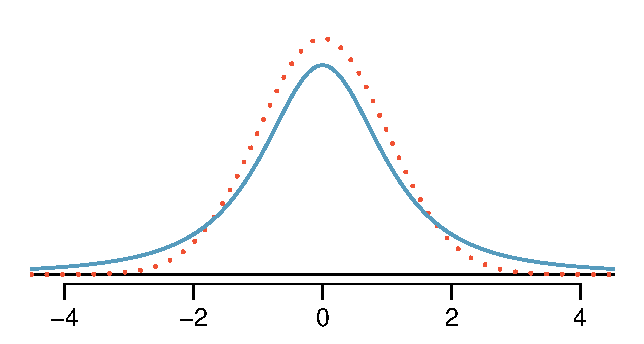
\includegraphics[height=45mm]{ch_inference_for_means/figures/tDistCompareToNormalDist/tDistCompareToNormalDist}
\caption{Comparison of a $t$ distribution (solid line) and a normal distribution (dotted line).}
\label{tDistCompareToNormalDist}
\end{figure}

The $t$ distribution, always centered at zero, has a single parameter: degrees of freedom. The \termsub{degrees of freedom (df)}{degrees of freedom (df)!$t$ distribution} describe the precise form of the bell-shaped $t$ distribution. Several $t$ distributions are shown in Figure~\ref{tDistConvergeToNormalDist}. When there are more degrees of freedom, the $t$~distribution looks very much like the standard normal distribution.

\begin{figure}
\centering
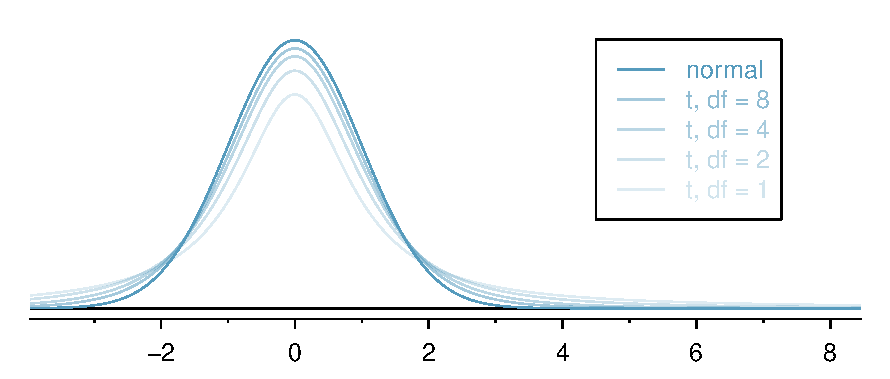
\includegraphics[width=0.8\textwidth]{ch_inference_for_means/figures/tDistConvergeToNormalDist/tDistConvergeToNormalDist}
\caption{The larger the degrees of freedom, the more closely the $t$ distribution resembles the standard normal model.}
\label{tDistConvergeToNormalDist}
\end{figure}

\begin{termBox}{\tBoxTitle{Degrees of freedom (df)}
The degrees of freedom describe the shape of the $t$ distribution. The larger the degrees of freedom, the more closely the distribution approximates the normal model.}
\end{termBox}

When the degrees of freedom is about 30 or more, the $t$ distribution is nearly indistinguishable from the normal distribution. In Section~\ref{tDistSolutionToSEProblem}, we relate degrees of freedom to sample size.

We will find it very useful to become familiar with the $t$ distribution, because it plays a very similar role to the normal distribution during inference for small samples of numerical data. We use a \term{t table}, partially shown in Table~\ref{tTableSample}, in place of the normal probability table for small sample numerical data. A larger table is presented in Appendix~\ref{tDistributionTable} on page~\pageref{tDistributionTable}. \Add{In~practice, it is also now standard to use statistical software instead of a table, and you can see some of these options at \href{https://openintro.org/stat/prob-tables}{openintro.org/stat/prob-tables}.} \Comment{Still need to create openintro.org/stat/prob-tables and tweak this link to have https:// etc. This type of note should also be added elsewhere in the textbook.}

\begin{table}[hht]
\centering
\begin{tabular}{r | rrr rr}
one tail & \hspace{1.5mm}  0.100 & \hspace{1.5mm} 0.050 & \hspace{1.5mm} 0.025 & \hspace{1.5mm} 0.010 & \hspace{1.5mm} 0.005  \\
two tails & 0.200 & 0.100 & 0.050 & 0.020 & 0.010 \\
\hline
{$df$} \hfill 1  &  {\normalsize  3.08} & {\normalsize  6.31} & {\normalsize 12.71} & {\normalsize 31.82} & {\normalsize 63.66}  \\ 
2  &  {\normalsize  1.89} & {\normalsize  2.92} & {\normalsize  4.30} & {\normalsize  6.96} & {\normalsize  9.92}  \\ 
3  &  {\normalsize  1.64} & {\normalsize  2.35} & {\normalsize  3.18} & {\normalsize  4.54} & {\normalsize  5.84}  \\ 
$\vdots$ & $\vdots$ &$\vdots$ &$\vdots$ &$\vdots$ & \\
17  &  {\normalsize  1.33} & {\normalsize  1.74} & {\normalsize  2.11} & {\normalsize  2.57} & {\normalsize  2.90}  \\ 
\highlightO{18}  &  \highlightO{\normalsize  1.33} & \highlightO{\normalsize  1.73} & \highlightO{\normalsize  2.10} & \highlightO{\normalsize  2.55} & \highlightO{\normalsize  2.88}  \\ 
19  &  {\normalsize  1.33} & {\normalsize  1.73} & {\normalsize  2.09} & {\normalsize  2.54} & {\normalsize  2.86}  \\ 
20  &  {\normalsize  1.33} & {\normalsize  1.72} & {\normalsize  2.09} & {\normalsize  2.53} & {\normalsize  2.85}  \\ 
$\vdots$ & $\vdots$ &$\vdots$ &$\vdots$ &$\vdots$ & \\
400  &  {\normalsize  1.28} & {\normalsize  1.65} & {\normalsize  1.97} & {\normalsize  2.34} & {\normalsize  2.59}  \\ 
500  &  {\normalsize  1.28} & {\normalsize  1.65} & {\normalsize  1.96} & {\normalsize  2.33} & {\normalsize  2.59}  \\ 
$\infty$  &  {\normalsize  1.28} & {\normalsize  1.64} & {\normalsize  1.96} & {\normalsize  2.33} & {\normalsize  2.58}  \\ 
\end{tabular}
\caption{An abbreviated look at the $t$ table. Each row represents a different $t$ distribution. The columns describe the cutoffs for specific tail areas. The row with $df=18$ has been \highlightO{highlighted}.}
\label{tTableSample}
\end{table}

Each row in the $t$ table represents a $t$ distribution with different degrees of freedom. The columns correspond to tail probabilities. For instance, if we know we are working with the $t$ distribution with $df=18$, we can examine row 18, which is \highlightO{highlighted} in Table~\ref{tTableSample}. If we want the value in this row that identifies the cutoff for an upper tail of 10\%, we can look in the column where \emph{one tail} is 0.100. This cutoff is 1.33. If we had wanted the cutoff for the lower 10\%, we would use -1.33. Just like the normal distribution, all $t$ distributions are symmetric.

\begin{example}{What proportion of the $t$ distribution with 18 degrees of freedom falls below -2.10?}
Just like a normal probability problem, we first draw the picture in Figure~\ref{tDistDF18LeftTail2Point10} and shade the area below -2.10. To find this area, we identify the appropriate row: $df=18$. Then we identify the column containing the absolute value of -2.10; it is the third column. Because we are looking for just one tail, we examine the top line of the table, which shows that a one tail area for a value in the third row corresponds to 0.025. About 2.5\% of the distribution falls below -2.10. In the next example we encounter a case where the exact $t$ value is not listed in the table.
\end{example}

\begin{figure}
\centering
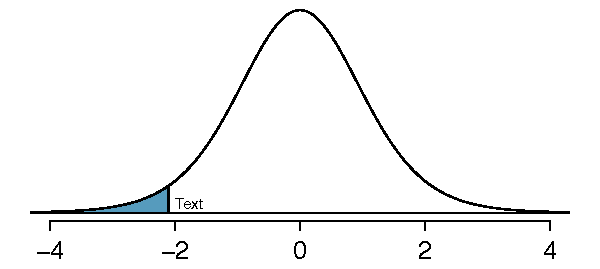
\includegraphics[width=0.55\textwidth]{ch_inference_for_means/figures/tDistDF18LeftTail2Point10/tDistDF18LeftTail2Point10}
\caption{The $t$ distribution with 18 degrees of freedom. The area below -2.10 has been shaded.}
\label{tDistDF18LeftTail2Point10}
\end{figure}

\begin{example}{A $t$ distribution with 20 degrees of freedom is shown in the left panel of Figure~\ref{tDistDF20RightTail1Point65}. Estimate the proportion of the distribution falling above 1.65.}
We identify the row in the $t$ table using the degrees of freedom: $df=20$. Then we look for 1.65; it is not listed. It falls between the first and second columns. Since these values bound 1.65, their tail areas will bound the tail area corresponding to 1.65. We identify the one tail area of the first and second columns, 0.050 and 0.10, and we conclude that between 5\% and 10\% of the distribution is more than 1.65 standard deviations above the mean. If we like, we can identify the precise area using statistical software: 0.0573.
\end{example}

\begin{figure}
\centering
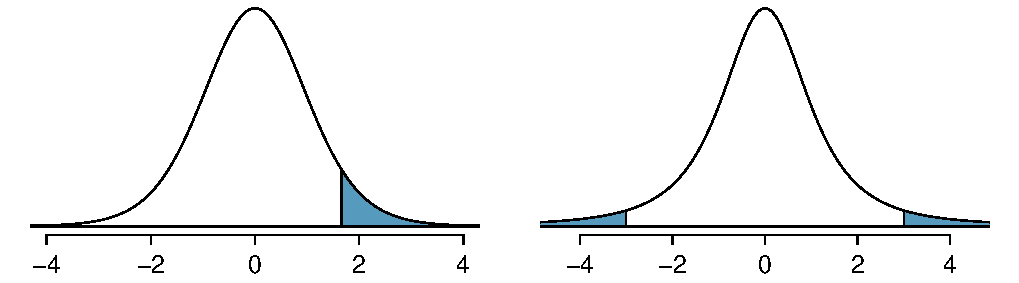
\includegraphics[width=0.85\textwidth]{ch_inference_for_means/figures/tDistDF20RightTail1Point65/tDistDF20RightTail1Point65}
\caption{Left: The $t$ distribution with 20 degrees of freedom, with the area above 1.65 shaded. Right: The $t$ distribution with 2 degrees of freedom, with the area further than 3 units from 0 shaded.}
\label{tDistDF20RightTail1Point65}
\end{figure}

\begin{example}{A $t$ distribution with 2 degrees of freedom is shown in the right panel of Figure~\ref{tDistDF20RightTail1Point65}. Estimate the proportion of the distribution falling more than 3 units from the mean (above or below).}
As before, first identify the appropriate row: $df=2$. Next, find the columns that capture 3; because $2.92 < 3 < 4.30$, we use the second and third columns. Finally, we find bounds for the tail areas by looking at the two tail values: 0.05 and 0.10. We use the two tail values because we are looking for two (symmetric) tails.
\end{example}

\begin{exercise}
What proportion of the $t$ distribution with 19 degrees of freedom falls above -1.79 units?\footnote{We find the shaded area \emph{above} -1.79 (we leave the picture to you). The small left tail is between 0.025 and 0.05, so the larger upper region must have an area between 0.95 and 0.975.}

\index{$t$ distribution|)}

\end{exercise}



\subsection{Conditions for using the $t$ distribution for inference on a sample mean}
\label{tDistSolutionToSEProblem}

\Comment{Revised the title of this subsection. It was previously ``The $t$ distribution as a solution to the standard error problem''.}

\Cut{When estimating the mean and standard error from a small sample, the $t$ distribution is a more accurate tool than the normal model. This is true for both small and large samples.}

%\Add{The $t$ distribution is a more accurate tool than the normal model when working with sample means. Its slightly thicker tails account for some of the imprecision in the standard error calculation, and this is especially important when working with smaller samples.}

To proceed with the $t$ distribution for inference about a single mean, we must check two conditions.
\begin{description}
\item[Independence of observations.] We verify this condition just as we did before. We collect a simple random sample from less than 10\% of the population, or if it was an experiment or random process, we carefully check to the best of our abilities that the observations were independent.
\item[Observations come from a nearly normal distribution.] This second condition is difficult to verify with small data sets. We often (i) take a look at a plot of the data for obvious departures from the normal model, and (ii) consider whether any previous experiences alert us that the data may not be nearly normal.
\end{description}
When examining a sample mean and estimated standard error from a sample of $n$ independent and nearly normal observations, we use a $t$ distribution with $n-1$ degrees of freedom~($df$). For example, if the sample size was 19, then we would use the $t$ distribution with $df=19-1=18$ degrees of freedom and proceed exactly as we did in Chapter~\ref{foundationsForInference}, except that \emph{now we use the $t$ \Add{distribution.}} \Cut{\emph{table}.}

\Comment{The tip box below was moved here from earlier in the subsection.}

\begin{tipBox}{\tipBoxTitle{When to use the $t$ distribution}
Use the $t$ distribution for inference of the sample mean when observations are independent and nearly normal. You may relax the nearly normal condition as the sample size increases. For example, the data distribution may be moderately skewed when the sample size is at least~30.
}
\end{tipBox}


\subsection{One sample $t$ confidence intervals}
\label{oneSampleTConfidenceIntervals}

\index{data!dolphins and mercury|(}

Dolphins are at the top of the oceanic food chain, which causes dangerous substances such as mercury to concentrate in their organs and muscles. This is an important problem for both dolphins and other animals, like humans, who occasionally eat them. For instance, this is particularly relevant in Japan where school meals have included dolphin at times.
\setlength{\captionwidth}{71.5mm}

\begin{figure}[h]
\centering
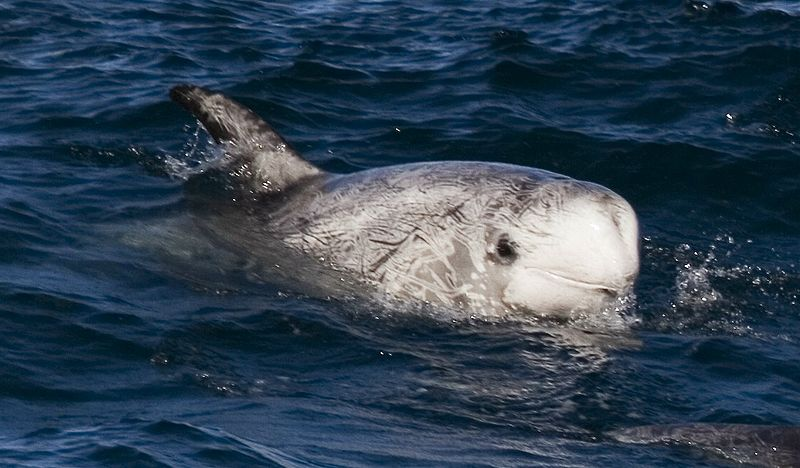
\includegraphics[width=0.65\textwidth]{ch_inference_for_means/figures/rissosDolphin/rissosDolphin.jpg}  \\
\addvspace{2mm}
\begin{minipage}{\textwidth}
   \caption[rissosDolphinPic]{A Risso's dolphin.\vspace{-1mm} \\
   -----------------------------\vspace{-2mm}\\
   {\footnotesize Photo by Mike Baird (\urlwofont{http://www.bairdphotos.com/}).%Image is under Creative Commons Attribution 2.0 Generic.
}\vspace{-8mm}}
   \label{rissosDolphin}
\end{minipage}
\vspace{3mm}
\end{figure}
\setlength{\captionwidth}{\mycaptionwidth}

Here we identify a confidence interval for the average mercury content in dolphin muscle using a sample of 19 Risso's dolphins from the Taiji area in Japan.\footnote{Taiji was featured in the movie \emph{The Cove}, and it is a significant source of dolphin and whale meat in Japan. Thousands of dolphins pass through the Taiji area annually, and we will assume these 19 dolphins represent a simple random sample from those dolphins. Data reference: Endo T and Haraguchi K. 2009. High mercury levels in hair samples from residents of Taiji, a Japanese whaling town. Marine Pollution Bulletin 60(5):743-747.} The data are summarized in Table~\ref{summaryStatsOfHgInMuscleOfRissosDolphins}. The minimum and maximum observed values can be used to evaluate whether or not there are obvious outliers or skew.

\begin{table}[h]
\centering
\begin{tabular}{ccc cc}
\hline
$n$ & $\bar{x}$ & $s$ & minimum & maximum \\
19   & 4.4	  & 2.3  & 1.7	       & 9.2 \\
\hline
\end{tabular}
\caption{Summary of mercury content in the muscle of 19 Risso's dolphins from the Taiji area. Measurements are in $\mu$g/wet g (micrograms of mercury per wet gram of muscle).}
\label{summaryStatsOfHgInMuscleOfRissosDolphins}
\end{table}

\begin{example}{Are the independence and normality conditions satisfied for this data~set?}
The observations are a simple random sample and consist of less than 10\% of the population, therefore independence is reasonable. The summary statistics in Table~\ref{summaryStatsOfHgInMuscleOfRissosDolphins} do not suggest any skew or outliers; all observations are within 2.5 standard deviations of the mean. Based on this evidence, the normality assumption seems reasonable.
\end{example}

In the normal model, we used $z^{\star}$ and the standard error to determine the width of a confidence interval. We revise the confidence interval formula slightly when using the $t$ distribution:
\begin{eqnarray*}
\bar{x} \ \pm\  t^{\star}_{df}SE
\end{eqnarray*}
\marginpar[\raggedright\vspace{-9mm}

$t^{\star}_{df}$\vspace{1mm}\\\footnotesize Multiplication\\factor for\\$t$ conf. interval]{\raggedright\vspace{-9mm}

$t^{\star}_{df}$\vspace{1mm}\\\footnotesize Multiplication\\factor for\\$t$ conf. interval}The sample mean and estimated standard error are computed just as before ($\bar{x} = 4.4$ and $SE = s/\sqrt{n} = 0.528$). The value $t^{\star}_{df}$ is a cutoff we obtain based on the confidence level and the $t$ distribution with $df$ degrees of freedom. Before determining this cutoff, we will first need the degrees of freedom.

\begin{termBox}{\tBoxTitle{Degrees of freedom for a single sample}
If the sample has $n$ observations and we are examining a single mean, then we use the $t$ distribution with $df=n-1$ degrees of freedom.}
\end{termBox}

In our current example, we should use the $t$ distribution with $df=19-1=18$ degrees of freedom. Then identifying $t_{18}^{\star}$ is similar to how we found $z^{\star}$. 
\begin{itemize}
\setlength{\itemsep}{0mm}
\item For a 95\% confidence interval, we want to find the cutoff $t^{\star}_{18}$ such that 95\% of the $t$ distribution is between -$t^{\star}_{18}$ and $t^{\star}_{18}$.
\item We look in the $t$ table on page~\pageref{tTableSample}, find the column with area totaling 0.05 in the two tails (third column), and then the row with 18 degrees of freedom: $t^{\star}_{18} = 2.10$.
\end{itemize}
Generally the value of $t^{\star}_{df}$ is slightly larger than what we would get under the normal model with~$z^{\star}$.



Finally, we can substitute all our values into the confidence interval equation to create the 95\% confidence interval for the average mercury content in muscles from Risso's dolphins that pass through the Taiji area:
\begin{eqnarray*}
\bar{x} \ \pm\  t^{\star}_{18}SE
	\quad \to \quad
4.4 \ \pm\  2.10 \times 0.528
	\quad \to \quad
(3.29, 5.51)
\end{eqnarray*}
We are 95\% confident the average mercury content of muscles in Risso's dolphins is between 3.29 and 5.51 $\mu$g/wet gram\Add{, which is considered extremely high}. \Cut{This is above the Japanese regulation level of 0.4 $\mu$g/wet gram.}

\index{data!dolphins and mercury|)}

\begin{termBox}{\tBoxTitle{Finding a $t$ confidence interval for the mean}
Based on a sample of $n$ independent and nearly normal observations, a confidence interval for the population mean is
\begin{eqnarray*}
\bar{x} \ \pm\  t^{\star}_{df}SE
\end{eqnarray*}
where $\bar{x}$ is the sample mean, $t^{\star}_{df}$ corresponds to the confidence level and degrees of freedom, and $SE$ is the standard error as estimated by the sample.}
\end{termBox}

\begin{exercise} \label{croakerWhiteFishPacificExerConditions}
\index{data!white fish and mercury|(}
The FDA's webpage provides some data on mercury content of fish.\footnote{\urlwofont{http://www.fda.gov/food/foodborneillnesscontaminants/metals/ucm115644.htm}} Based on a sample of 15 croaker white fish (Pacific), a sample mean and standard deviation were computed as 0.287 and 0.069 ppm (parts per million), respectively. The 15 observations ranged from 0.18 to 0.41 ppm. We will assume these observations are independent. Based on the summary statistics of the data, do you have any objections to the normality condition of the individual observations?\footnote{There are no obvious outliers; all observations are within 2 standard deviations of the mean. If there is skew, it is not evident. There are no red flags for the normal model based on this (limited) information, and we do not have reason to believe the mercury content is not nearly normal in this type of fish.}
\end{exercise}

\begin{example}{Estimate the standard error of $\bar{x}=0.287$ ppm using the data summaries in Exercise~\ref{croakerWhiteFishPacificExerConditions}. If we are to use the $t$ distribution to create a 90\% confidence interval for the actual mean of the mercury content, identify the degrees of freedom we should use and also find $t^{\star}_{df}$.}
\label{croakerWhiteFishPacificExerSEDFTStar}
The standard error: $SE = \frac{0.069}{\sqrt{15}} = 0.0178$. Degrees of freedom: $df = n - 1 = 14$.

Looking in the column where two tails is 0.100 (for a 90\% confidence interval) and row $df=14$, we identify $t^{\star}_{14} = 1.76$.
\end{example}

\begin{exercise}
Using the results of Exercise~\ref{croakerWhiteFishPacificExerConditions} and Example~\ref{croakerWhiteFishPacificExerSEDFTStar}, compute a 90\% confidence interval for the average mercury content of croaker white fish (Pacific).\footnote{$\bar{x} \ \pm\ t^{\star}_{14} SE \ \to\  0.287 \ \pm\  1.76\times 0.0178\ \to\ (0.256, 0.318)$. We are 90\% confident that the average mercury content of croaker white fish (Pacific) is between 0.256 and 0.318 ppm.}

\index{data!white fish and mercury|)}

\end{exercise}



\subsection{One sample $t$ tests}
\label{oneSampleTTests}

\Comment{This section is from ISRS. This should either be rewritten to have a different application or the context of Chapter 4 should be changed (or both).}

Is the typical US runner getting faster or slower over time? We consider this question in the context of the Cherry Blossom Run, comparing runners in 2006 and 2012. Technological advances in shoes, training, and diet might suggest runners would be faster in 2012. An opposing viewpoint might say that \Cut{with the average body mass index on the rise, people tend to run slower.} \Add{Americans (who make up most of the runners) have become less healthy, so the participants will tend to run slower.} In fact, all of these components might be influencing \Add{the average} run time.

The average time for all runners who finished the Cherry Blossom Run in 2006 was 93.29 minutes (93 minutes and about 17 seconds). We want to determine using data from 100 participants in the 2012 Cherry Blossom Run whether runners in this race are getting faster or slower, versus the other possibility that there has been no change.

\begin{exercise}
What are appropriate hypotheses for this context?\footnote{$H_0$: The average 10 mile run time was the same for 2006 and 2012. $\mu = 93.29$ minutes. $H_A$: The average 10 mile run time for 2012 was \emph{different} than that of 2006. $\mu \neq 93.29$ minutes.}
\end{exercise}

\begin{exercise}
The data come from a simple random sample from less than 10\% of all participants, so the observations are independent. However, should we be worried about skew in the data? A histogram of the differences \Add{is shown in Figure~\ref{run10SampTimeHistogram}.} \Cut{was shown in the left panel of Figure~\vref{run10SampHistograms}.}~\footnote{With a sample of 100, we should only be concerned if there is extreme skew. The histogram of the data suggest, at worst, slight skew.} \Comment{The caption to the figure was revised.}
\end{exercise}

\begin{figure}[h]
\centering
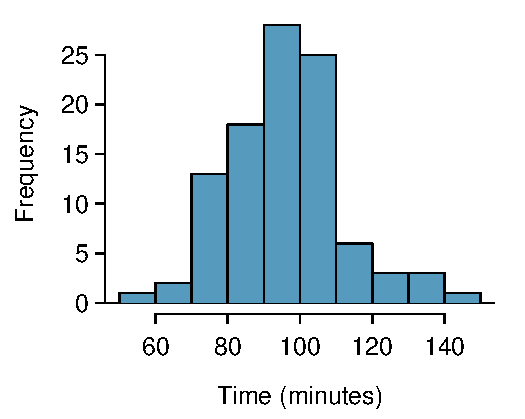
\includegraphics[width=0.45\textwidth]{ch_inference_for_means/figures/run10SampTimeHistogram/run10SampTimeHistogram} 
\caption{A histogram of \var{time} for the sample Cherry Blossom Run data.}
\label{run10SampTimeHistogram}
\end{figure}

With independence satisfied and \Add{slight} skew not a concern \Add{for this large of a sample}, we can proceed with performing a hypothesis test using the $t$ distribution.

\begin{exercise}
The sample mean and sample standard deviation are 95.61 and 15.78 minutes, respectively. Recall that the sample size is 100. What is the p-value for the test, and what is your conclusion?\footnote{With the conditions satisfied for the $t$ distribution, we can compute the standard error ($SE = 15.78 / \sqrt{100} = 1.58$ and the \emph{T score}: $T = \frac{95.61 - 93.29}{1.58} = 1.47$. (There is more on this after the guided practice, but a T score and Z score are basically the same thing.) For $df = 100 - 1 = 99$, we would find $T = 1.47$ to fall between the first and second column, which means the p-value is between 0.10 and 0.20 (use $df = 90$ and consider two tails since the test is two-sided). The p-value could also have been calculated more precisely with statistical software: 0.1447. Because the p-value is greater than 0.05, we do not reject the null hypothesis. That is, the data do not provide strong evidence that the average run time for the Cherry Blossom Run in 2012 is any different than the 2006 average.}
\end{exercise}

\begin{termBox}{\tBoxTitle{When using a $t$ distribution, we use a T score (same as Z score)}
To help us remember to use the $t$ distribution, we use a $T$ to represent the test statistic, and we often call this a \term{T score}. The Z score and T score are computed in the exact same way and are conceptually identical: each represents how many standard errors the observed value is from the null value.}
\end{termBox}



%__________________
\section{Paired data}
\label{pairedData}

\Comment{This section was pulled from ISRS.}

\index{paired data|(}
\index{data!textbooks|(}

Are textbooks actually cheaper online? Here we compare the price of textbooks at the University of California, Los Angeles' (UCLA's) bookstore and prices at Amazon.com. Seventy-three UCLA courses were randomly sampled in Spring 2010, representing less than 10\% of all UCLA courses.\footnote{When a class had multiple books, only the most expensive text was considered.} A portion of the data set is shown in Table~\ref{textbooksDF}.

\begin{table}[h]
\centering
\begin{tabular}{rllrrr}
  \hline
 & dept & course & ucla & amazon & diff \\ 
  \hline
1 & Am Ind &  C170 & 27.67 & 27.95 & -0.28 \\ 
  2 & Anthro & 9 & 40.59 & 31.14 & 9.45 \\ 
  3 & Anthro & 135T & 31.68 & 32.00 & -0.32 \\ 
  4 & Anthro & 191HB & 16.00 & 11.52 & 4.48 \\ 
$\vdots$ & $\vdots$ & $\vdots$ & $\vdots$ & $\vdots$ & $\vdots$ \\
  72 & Wom Std & M144 & 23.76 & 18.72 & 5.04 \\ 
  73 & Wom Std & 285 & 27.70 & 18.22 & 9.48 \\ 
   \hline
\end{tabular}
\caption{Six cases of the \data{textbooks} data set.}
\label{textbooksDF}
\end{table}
%library(openintro); library(xtable); data(textbooks); xtable(textbooks[c(1:5, nrow(textbooks) - 1:0),])

\subsection{Paired observations}

Each textbook has two corresponding prices in the data set: one for the UCLA bookstore and one for Amazon. Therefore, each textbook price from the UCLA bookstore has a natural correspondence with a textbook price from Amazon. When two sets of observations have this special correspondence, they are said to be \term{paired}.

\begin{termBox}{\tBoxTitle{Paired data}
Two sets of observations are \emph{paired} if each observation in one set has a special correspondence or connection with exactly one observation in the other data set.}
\end{termBox}

To analyze paired data, it is often useful to look at the difference in outcomes of each pair of observations. In the \data{textbook} data set, we look at the difference in prices, which is represented as the \var{diff} variable in the \data{textbooks} data. Here the differences are taken as
\begin{eqnarray*}
\text{UCLA price} - \text{Amazon price}
\end{eqnarray*}
for each book. It is important that we always subtract using a consistent order; here Amazon prices are always subtracted from UCLA prices. A histogram of these differences is shown in Figure~\ref{diffInTextbookPricesS10}. Using differences between paired observations is a common and useful way to analyze paired data.

\begin{figure}
\centering
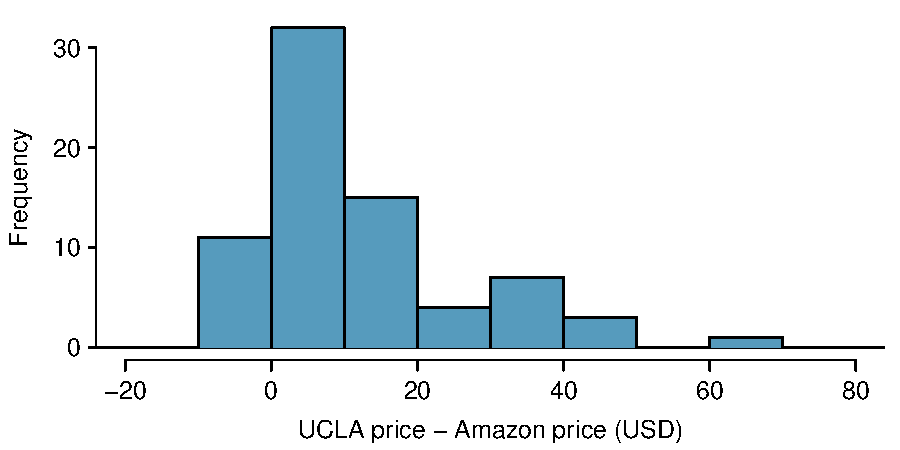
\includegraphics[width=0.87\textwidth]{ch_inference_for_means/figures/textbooksS10/diffInTextbookPricesS10}
\caption{Histogram of the difference in price for each book sampled. These data are strongly skewed.\index{skew!example: strong}}
\label{diffInTextbookPricesS10}
\end{figure}

\begin{exercise}
The first difference shown in Table~\ref{textbooksDF} is computed as $27.67-27.95=-0.28$. Verify the differences are calculated correctly for observations~2 and~3.\footnote{Observation 2: $40.59 - 31.14 = 9.45$. Observation 3: $31.68 - 32.00 = -0.32$.}
\end{exercise}


\subsection{Inference for paired data}

To analyze a paired data set, we simply analyze the differences. We can use the same $t$~distribution techniques we applied in the last section.

\begin{table}[hh]
\centering
\begin{tabular}{ccccc}
\hline
$n_{_{diff}}$	&\hspace{3mm}& $\bar{x}_{_{diff}}$	&\hspace{3mm}& $s_{_{diff}}$ \vspace{1mm}\\
73			&& 12.76				&& 14.26 \\
\hline
\end{tabular}
\caption{Summary statistics for the price differences. There were 73 books, so there are 73 differences.}
\label{textbooksSummaryStats}
\end{table}

\begin{example}{Set up and implement a hypothesis test to determine whether, on average, there is a difference between Amazon's price for a book and the UCLA bookstore's price.}
\label{htForDiffInUCLAAndAmazonTextbookPrices}
We are considering two scenarios: there is no difference or there is some difference in average prices.
\begin{itemize}
\setlength{\itemsep}{0mm}
\item[$H_0$:] $\mu_{diff}=0$. There is no difference in the average textbook price.
\item[$H_A$:] $\mu_{diff} \neq 0$. There is a difference in average prices.
\end{itemize}

Can the $t$ distribution be used for this application? The observations are based on a simple random sample from less than 10\% of all books sold at the bookstore, so independence is reasonable. While the distribution is strongly skewed, the sample is reasonably large ($n=73$), so we can proceed. Because the conditions are reasonably satisfied, we can apply the $t$ distribution to this setting.

We compute the standard error associated with $\bar{x}_{diff}$ using the standard deviation of the differences ($s_{_{diff}}=14.26$) and the number of differences ($n_{_{diff}}=73$):
$$SE_{\bar{x}_{diff}} = \frac{s_{diff}}{\sqrt{n_{diff}}} = \frac{14.26}{\sqrt{73}} = 1.67$$
To visualize the p-value, the sampling distribution of $\bar{x}_{diff}$ is drawn as though $H_0$ is true, which is shown in Figure~\ref{textbooksS10HTTails}. The p-value is represented by the two (very) small tails.

To find the tail areas, we compute the test statistic, which is the T score of $\bar{x}_{diff}$ under the null condition that the actual mean difference is 0:
$$T = \frac{\bar{x}_{diff} - 0}{SE_{x_{diff}}} = \frac{12.76 - 0}{1.67} = 7.59$$
The degrees of freedom are $df = 73 - 1 = 72$. If we examined Appendix~\vref{tDistributionTable}, we would see that this value is larger than any in the 70 df row (we round down for $df$ when using the table), meaning the two-tailed p-value is less than 0.01. If we used statistical software, we would find the p-value is less than 1-in-10 billion! Because the p-value is less than 0.05, we reject the null hypothesis. We have found convincing evidence that Amazon \Cut{is} \Add{was}, on average, cheaper than the UCLA bookstore for UCLA course textbooks.
\end{example}

\begin{figure}[h]
\centering
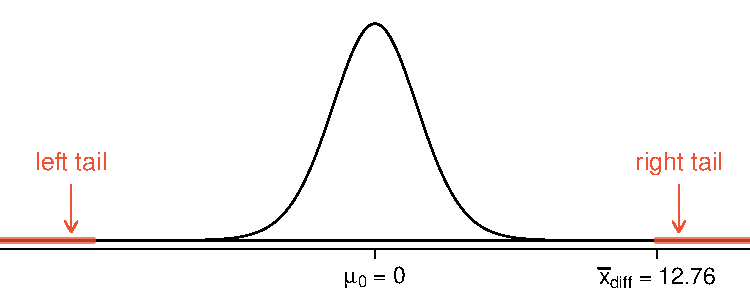
\includegraphics[width=0.65\textwidth]{ch_inference_for_means/figures/textbooksS10/textbooksS10HTTails}
\caption{Sampling distribution for the mean difference in book prices, if the true average difference is zero.}
\label{textbooksS10HTTails}
\end{figure}

\begin{exercise}
Create a 95\% confidence interval for the average price difference between books at the UCLA bookstore and books on Amazon.\footnote{Conditions have already verified and the standard error computed in Example~\ref{htForDiffInUCLAAndAmazonTextbookPrices}. To find the interval, identify $t^{\star}_{72}$ (use $df=70$ in the table, $t^{\star}_{70} = 1.99$) and plug it, the point estimate, and the standard error into the confidence interval formula:
$$\text{point estimate} \ \pm\ z^{\star}SE \quad\to\quad 12.76 \ \pm\ 1.99\times 1.67 \quad\to\quad (9.44, 16.08)$$
We are 95\% confident that Amazon is, on average, between \$9.44 and \$16.08 cheaper than the UCLA bookstore for UCLA course books.}

\index{data!textbooks|)}
\index{paired data|)}

\end{exercise}

\Cut{In the textbook price example, we applied the $t$ distribution. However, as we mentioned in the last section, the $t$ distribution looks a lot like the normal distribution when the degrees of freedom are larger than about 30. In such cases, including this one, it would be reasonable to use the normal distribution in place of the $t$ distribution.}



%__________________
\section{Difference of two means}
\label{differenceOfTwoMeans}

{
In this section we consider a difference in two population means, $\mu_1 - \mu_2$, under the condition that the data are not paired. Just as with a single sample, we identify conditions to ensure we can use the $t$ distribution with a point estimate of the difference, $\bar{x}_1 - \bar{x}_2$.

We apply these methods in three contexts: determining whether stem cells can improve heart function, exploring the impact of pregnant womens' smoking habits on birth weights of newborns, and exploring whether there is statistically significant evidence that one variations of an exam is harder than another variation. This section is motivated by questions like ``Is there convincing evidence that newborns from mothers who smoke have a different average birth weight than newborns from mothers who don't smoke?''

\subsection{Confidence interval for a differences of means}

\index{data!stem cells, heart function|(}
\index{point estimate!difference of means|(}

Does treatment using embryonic stem cells (ESCs) help improve heart function following a heart attack? Table~\ref{summaryStatsForSheepHeartDataWhoReceivedMiceESCs} contains summary statistics for an experiment to test ESCs in sheep that had a heart attack. Each of these sheep was randomly assigned to the ESC or control group, and the change in their hearts' pumping capacity was measured in the study. A~positive value corresponds to increased pumping capacity, which generally suggests a stronger recovery. Our goal will be to identify a 95\% confidence interval for the effect of ESCs on the change in heart pumping capacity relative to the control group.

A point estimate of the difference in the heart pumping variable can be found using the difference in the sample means:
\begin{eqnarray*}
\bar{x}_{esc} - \bar{x}_{control}\ =\ 3.50 - (-4.33)\ =\ 7.83
\end{eqnarray*}

\begin{table}[h]
\centering
\begin{tabular}{l rrrrr}
\hline
\hspace{10mm}	& $n$	& $\bar{x}$	& $s$  	 \\
\hline
ESCs		& 9		& 3.50		& 5.17  	\\
control		& 9		& -4.33		& 2.76  	 \\
\hline
\end{tabular}
\caption{Summary statistics of the embryonic stem cell study.}
\label{summaryStatsForSheepHeartDataWhoReceivedMiceESCs}
\end{table}

\begin{figure}[h]
\centering
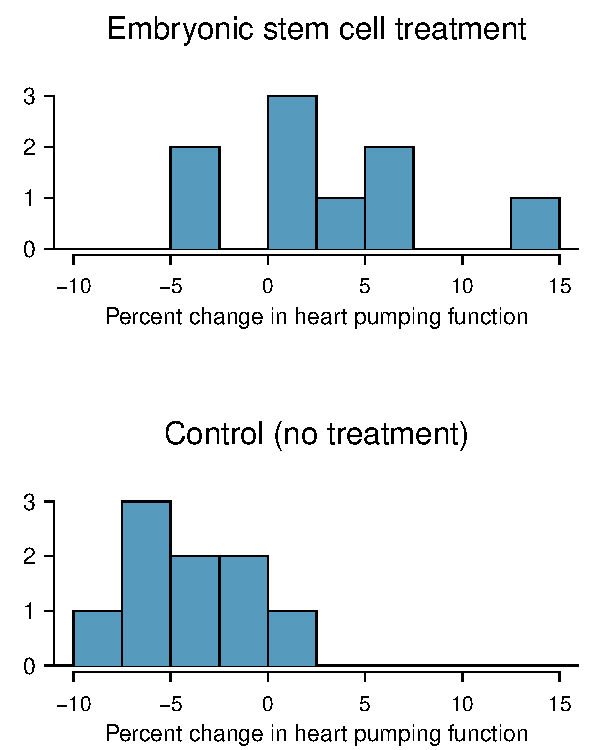
\includegraphics[width=0.6\textwidth]{ch_inference_for_means/figures/stemCellTherapyForHearts/stemCellTherapyForHearts}
\caption{Histograms for both the embryonic stem cell group and the control group. Higher values are associated with greater improvement. We don't see any evidence of skew in these data; however, it is worth noting that skew would be difficult to detect with such a small sample.}
\label{stemCellTherapyForHearts}
\end{figure}

%\begin{example}{Set up hypotheses that will be used to test whether there is convincing evidence that ESCs actually increase the amount of blood the heart pumps. Also, check conditions for using the $t$ distribution for inference with the point estimate $\bar{x}_1 - \bar{x}_2$. To assist in this assessment, the data are presented in Figure~\ref{stemCellTherapyForHearts}.}\label{exampleToEvaluteWhetherESCsAreHelpfulInImprovingHeartFunctionInSheep}
%We first setup the hypotheses:
%\begin{itemize}
%\setlength{\itemsep}{0mm}
%\item[$H_0$:] The stem cells do not improve heart pumping function. $\mu_{esc} - \mu_{control} = 0$.
%\item[$H_A$:] The stem cells do improve heart pumping function. $\mu_{esc} - \mu_{control} > 0$.
%\end{itemize}
%\end{example}

\begin{termBox}{\tBoxTitle{Using the $t$ distribution for a difference in means}
\label{ConditionsForTwoSampleTDist}The $t$ distribution can be used for inference when working with the standardized difference of two means if (1) each sample meets the conditions for using the $t$ distribution and (2) the samples are independent.}
\end{termBox}

\begin{example}{Can the point estimate, $\bar{x}_{esc} - \bar{x}_{control} = 7.83$, be analyzed using the $t$ distribution?}
We check the two required conditions: % the $t$ distribution can be used by (1) checking whether each sample mean could itself be modeled using the $t$ distribution and (2) determining whether the samples are independent.
\begin{enumerate}
\item In this study, the sheep were independent of each other. Additionally, the distributions in Figure~\ref{stemCellTherapyForHearts} don't show any clear deviations from normality, where we watch for prominent outliers in particular for such small samples. These findings imply each sample mean could itself be modeled using a $t$ distribution.
\item The sheep in each group were also independent of each other.
\end{enumerate}
Because both conditions are met, we can use the $t$ distribution to model the difference of the two sample means.
\end{example}

%\begin{termBox}{\tBoxTitle{Conditions for applying the $t$ distribution to $\bar{x}_1 - \bar{x}_2$}
%If the sample means, $\bar{x}_1$ and $\bar{x}_2$, each meet the criteria for using the $t$ distribution and the observations in the two samples are independent, then we can analyze the difference in sample means using the $t$ distribution.}
%\end{termBox}

\index{point estimate!difference of means|)}

\index{standard error!difference in means}
\Add{
We can quantify the variability in the point estimate, $\bar{x}_{esc} - \bar{x}_{control}$, using the following formula for its standard error:
\index{standard error!difference in means}
\begin{eqnarray*}
SE_{\bar{x}_{esc} - \bar{x}_{control}} = \sqrt{\frac{\sigma_{esc}^2}{n_{esc}} + \frac{\sigma_{control}^2}{n_{control}}}
\end{eqnarray*}
We usually estimate this standard error using standard deviation estimates  based on the samples:
}

\Cut{Before we construct a confidence interval, we must calculate the standard error of the point estimate of the difference. For this, we use the following formula, where just as before we substitute the sample standard deviations into the formula:}
% We can quantify the variability in the point estimate, $\bar{x}_{esc} - \bar{x}_{control}$, using the following formula for its standard error:
%\begin{eqnarray*}
%SE_{\bar{x}_{esc} - \bar{x}_{control}} = \sqrt{\frac{\sigma_{esc}^2}{n_{esc}} + \frac{\sigma_{control}^2}{n_{control}}}
%\end{eqnarray*}
%We usually estimate this standard error using standard deviation estimates  based on the samples:
\begin{align*}
SE_{\bar{x}_{esc} - \bar{x}_{control}}
	&= \sqrt{\frac{\sigma_{esc}^2}{n_{esc}} + \frac{\sigma_{control}^2}{n_{control}}} \\
	&\approx \sqrt{\frac{s_{esc}^2}{n_{esc}} + \frac{s_{control}^2}{n_{control}}}
	= \sqrt{\frac{5.17^2}{9} + \frac{2.76^2}{9}} = 1.95
\end{align*}
Because we will use the $t$ distribution, we also must identify the appropriate degrees of freedom. This can be done using computer software. An alternative technique is to use the smaller of $n_1 - 1$ and $n_2 - 1$, which is the method we will typically apply in the examples and guided practice.\footnote{This technique for degrees of freedom is conservative with respect to a Type 1 Error; it is more difficult to reject the null hypothesis using this $df$ method. In this example, computer software would have provided us a more precise degrees of freedom of $df = 12.225$.}

\begin{termBox}{\tBoxTitle{Distribution of a difference of sample means}
The sample difference of two means, $\bar{x}_1 - \bar{x}_2$, can be modeled using the $t$ distribution and the standard error
\begin{eqnarray}
\textstyle
SE_{\bar{x}_{1} - \bar{x}_{2}} = \sqrt{\frac{s_1^2}{n_1} + \frac{s_2^2}{n_2}}
\label{seOfDifferenceInMeans}
\end{eqnarray}
when each sample mean can itself be modeled using a $t$ distribution and the samples are independent. To calculate the degrees of freedom, use statistical software or the smaller of $n_1 - 1$ and $n_2 - 1$.}
\end{termBox}

\begin{example}{Calculate a 95\% confidence interval for the effect of ESCs on the change in heart pumping capacity of sheep after they've suffered a heart attack.}
We will use the sample difference and the standard error for that point estimate from our earlier calculations:
\begin{align*}
& \bar{x}_{esc} - \bar{x}_{control} = 7.83 \\
& SE = \sqrt{\frac{5.17^2}{9} + \frac{2.76^2}{9}} = 1.95
\end{align*}
Using $df = 8$, we can identify the appropriate $t^{\star}_{df} = t^{\star}_{8}$ for a 95\% confidence interval as 2.31. Finally, we can enter the values into the confidence interval formula:
\begin{align*}
\text{point estimate} \ \pm\ z^{\star}SE \quad\rightarrow\quad
7.83 \ \pm\ 2.31\times 1.95 \quad\rightarrow\quad (3.38, 12.38)
\end{align*}
We are 95\% confident that embryonic stem cells improve the heart's pumping function in sheep that have suffered a heart attack by 3.38\% to 12.38\%.
\end{example}

\index{data!stem cells, heart function|)}


\subsection{Hypothesis tests based on a difference in means}

\index{data!baby\_smoke|(}

A data set called \data{baby\_\hspace{0.3mm}smoke} represents a random sample of 150 cases of mothers and their newborns in North Carolina over a year. Four cases from this data set are represented in Table~\ref{babySmokeDF}. We are particularly interested in two variables: \var{weight} and \var{smoke}. The \var{weight} variable represents the weights of the newborns and the \var{smoke} variable describes which mothers smoked during pregnancy. We would like to know, is there convincing evidence that newborns from mothers who smoke have a different average birth weight than newborns from mothers who don't smoke? We will use the North Carolina sample to try to answer this question. The smoking group includes 50 cases and the nonsmoking group contains 100 cases, represented in Figure~\ref{babySmokePlotOfTwoGroupsToExamineSkew}.

\begin{table}[h]
\centering
\begin{tabular}{rrrrrll}
  \hline
 & fAge & mAge & weeks & weight & sexBaby & smoke \\ 
  \hline
1 & NA & 13 &  37 & 5.00 & female & nonsmoker \\ 
  2 & NA & 14 &  36 & 5.88 & female & nonsmoker \\ 
  3 & 19 & 15 &  41 & 8.13 & male & smoker \\ 
  $\vdots$ &   $\vdots$ &   $\vdots$ &   $\vdots$ &   $\vdots$ &   $\vdots$ \\
  150 & 45 & 50 &  36 & 9.25 & female & nonsmoker \\ 
   \hline
\end{tabular}
\caption{Four cases from the \data{baby\_\hspace{0.3mm}smoke} data set. The value ``NA'', shown for the first two entries of the first variable, indicates that piece of data is missing.}
\label{babySmokeDF}
\end{table}

\begin{figure}[hhh]
\centering
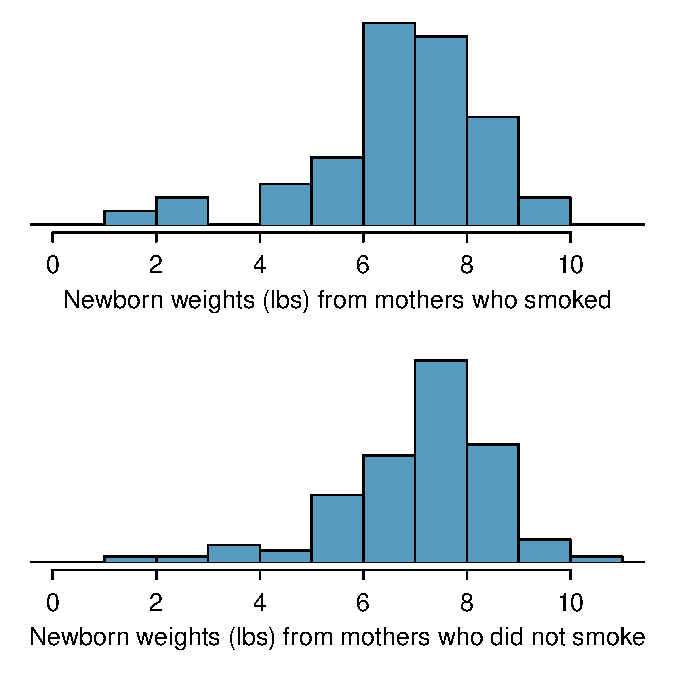
\includegraphics[width=0.6\textwidth]{ch_inference_for_means/figures/babySmokePlotOfTwoGroupsToExamineSkew/babySmokePlotOfTwoGroupsToExamineSkew}
\caption{The top panel represents birth weights for infants whose mothers smoked. The bottom panel represents the birth weights for infants whose mothers who did not smoke. The distributions exhibit moderate-to-strong and strong~skew, respectively.\index{skew!example: strong}}
\label{babySmokePlotOfTwoGroupsToExamineSkew}
\end{figure}

\begin{example}{Set up appropriate hypotheses to evaluate whether there is a relationship between a mother smoking and average birth weight.}\label{babySmokeHTForWeight}
The null hypothesis represents the case of no difference between the groups.
\begin{itemize}
\setlength{\itemsep}{0mm}
\item[$H_0$:] There is no difference in average birth weight for newborns from mothers who did and did not smoke. In statistical notation: $\mu_{n} - \mu_{s} = 0$, where $\mu_{n}$ represents non-smoking mothers and $\mu_s$ represents mothers who smoked.
\item[$H_A$:] There is some difference in average newborn weights from mothers who did and did not smoke ($\mu_{n} - \mu_{s} \neq 0$).
\end{itemize}
\end{example}

We check the two conditions necessary to apply the $t$ distribution to the difference in sample means. (1) Because the data come from a simple random sample and consist of less than 10\% of all such cases, the observations are independent. Additionally, while each distribution is strongly skewed, the sample sizes of 50 and 100 would make it reasonable to model each mean separately using a $t$ distribution. The skew is reasonable for these sample sizes of 50 and 100. (2) The independence reasoning applied in (1) also ensures the observations in each sample are independent. Since both conditions are satisfied, the difference in sample means may be modeled using a $t$ distribution.

%Summary statistics are shown for each sample in Table~\ref{summaryStatsOfBirthWeightForNewbornsFromSmokingAndNonsmokingMothers}.

\begin{table}[hhh]
\centering
\begin{tabular}{lrr}
	& \resp{smoker} & \resp{nonsmoker} \\
\hline
mean & 6.78 & 7.18 \\
st. dev. & 1.43 & 1.60 \\
samp. size & 50 & 100 \\
\hline
\end{tabular}
\caption{Summary statistics for the \data{baby\_\hspace{0.3mm}smoke} data set.}
\label{summaryStatsOfBirthWeightForNewbornsFromSmokingAndNonsmokingMothers}
\end{table}

\begin{exercise}
The summary statistics in Table~\ref{summaryStatsOfBirthWeightForNewbornsFromSmokingAndNonsmokingMothers} may be useful for this exercise. (a)~What is the point estimate of the population difference, $\mu_{n} - \mu_{s}$? (b)~Compute the standard error of the point estimate from part (a).\footnote{(a)~The difference in sample means is an appropriate point estimate: $\bar{x}_{n} - \bar{x}_{s} = 0.40$. (b)~The standard error of the estimate can be estimated using Equation~(\ref{seOfDifferenceInMeans}):
\begin{eqnarray*}
SE = \sqrt{\frac{\sigma_n^2}{n_n} + \frac{\sigma_s^2}{n_s}}
	\approx \sqrt{\frac{s_n^2}{n_n} + \frac{s_s^2}{n_s}}
	= \sqrt{\frac{1.60^2}{100} + \frac{1.43^2}{50}}
	= 0.26
\end{eqnarray*}}
\end{exercise}

\begin{example}{Draw a picture to represent the p-value for the hypothesis test from Example~\ref{babySmokeHTForWeight}.} \label{pictureOfPValueForEstimateOfDiffOfMeansOfBirthWeights}
To depict the p-value, we draw the distribution of the point estimate as though $H_0$ were true and shade areas representing at least as much evidence against $H_0$ as what was observed. Both tails are shaded because it is a two-sided test.
\begin{center}
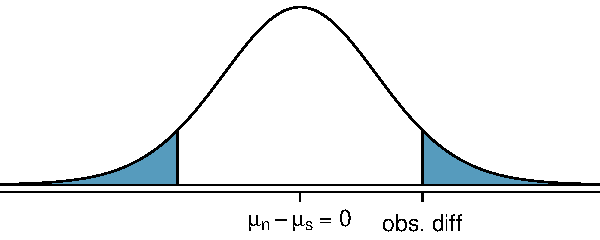
\includegraphics[width=0.6\textwidth]{ch_inference_for_means/figures/distOfDiffOfSampleMeansForBWOfBabySmokeData/distOfDiffOfSampleMeansForBWOfBabySmokeData}
\end{center}
\end{example}

\begin{example}{Compute the p-value of the hypothesis test using the figure in Example~\ref{pictureOfPValueForEstimateOfDiffOfMeansOfBirthWeights}, and evaluate the hypotheses using a significance level of $\alpha=0.05$.} \label{babySmokeHTForWeightComputePValueAndEvalHT}
We start by computing the T score:
\begin{eqnarray*}
T = \frac{\ 0.40 - 0\ }{0.26} = 1.54
\end{eqnarray*}
Next, we compare this value to values in the $t$ table in Appendix~\vref{tDistributionTable}, where we use the smaller of $n_n - 1 = 99$ and $n_s - 1 = 49$ as the degrees of freedom: $df = 49$. The T score falls between the first and second columns in the $df = 49$ row of the $t$ table, meaning the two-tailed p-value falls between 0.10 and 0.20 (reminder, find tail areas along the top of the table). This p-value is larger than the significance value, 0.05, so we fail to reject the null hypothesis. There is insufficient evidence to say there is a difference in average birth weight of newborns from North Carolina mothers who did smoke during pregnancy and newborns from North Carolina mothers who did not smoke during pregnancy.
\end{example}

\begin{exercise}
Does the conclusion to Example~\ref{babySmokeHTForWeightComputePValueAndEvalHT} mean that smoking and average birth weight are unrelated?\footnote{Absolutely not. It is possible that there is some difference but we did not detect it. If there is a difference, we made a Type 2 Error. Notice: we also don't have enough information to, if there is an actual difference difference, confidently say which direction that difference would be in.}
\end{exercise}

\begin{exercise} \label{babySmokeHTIDingHowToDetectDifferences}
If we made a Type 2 Error and there is a difference, what could we have done differently in data collection to be more likely to detect such a difference?\footnote{We could have collected more data. If the sample sizes are larger, we tend to have a better shot at finding a difference if one exists.}

\end{exercise}

\Add{Public service announcement: while we have used this relatively small data set as an example, larger data sets show that women who smoke tend to have smaller newborns. In~fact, some in the tobacco industry actually had the audacity to tout that as a \emph{benefit} of~smoking:
\begin{quotation}
\noindent\emph{It's true. The babies born from women who smoke are smaller, but they're just as healthy as the babies born from women who do not smoke. And some women would prefer having smaller babies.} \\[2mm]
\indent\indent\indent\indent\indent\indent- Joseph Cullman, Philip Morris' Chairman of the Board \\
\indent\indent\indent\indent\indent\indent{\color{white}...}on CBS' \emph{Face the Nation}, Jan 3,~1971
\end{quotation}
Fact check: the babies from women who smoke are not actually as healthy as from women who do not smoke.\footnote{You can watch an episode of John Oliver on \emph{This Week Tonight} to explore the present day offenses of the tobacco industry. Please be aware that there is some adult language: \href{http://youtube.com/watch?v=6UsHHOCH4q8}{youtube.com/watch?v=6UsHHOCH4q8}.} \Comment{The video in the footnote is unconventional for a textbook. Thoughts?}}
% Resource on this topic:
% http://archive.tobacco.org/Documents/documentquotes.html

\index{data!baby\_smoke|)}


\subsection{Case study: two versions of a course exam}

\index{data!two exam comparison|(}

An instructor decided to run two slight variations of the same exam. Prior to passing out the exams, she shuffled the exams together to ensure each student received a random version. Summary statistics for how students performed on these two exams are shown in Table~\ref{summaryStatsForTwoVersionsOfExams}. Anticipating complaints from students who took Version~B, she would like to evaluate whether the difference observed in the groups is so large that it provides convincing evidence that Version~B was more difficult (on average) than Version~A.

\begin{table}[hht]
\centering
\begin{tabular}{l rrrrr}
\hline
Version\hspace{2mm}	& $n$	& $\bar{x}$	& $s$	& min	& max  \\
\hline
A		& 30		& 79.4		& 14 	& 45		& 100 \\
B		& 27		& 74.1		& 20		& 32		& 100 \\
\hline
\end{tabular}
\caption{Summary statistics of scores for each exam version.}
\label{summaryStatsForTwoVersionsOfExams}
\end{table}

\begin{exercise} \label{htSetupForEvaluatingTwoExamVersions}
Construct a hypotheses to evaluate whether the observed difference in sample means, $\bar{x}_A - \bar{x}_B=5.3$, is due to chance.\footnote{Because the teacher did not expect one exam to be more difficult prior to examining the test results, she should use a two-sided hypothesis test. $H_0$: the exams are equally difficult, on average. $\mu_A - \mu_B = 0$. $H_A$: one exam was more difficult than the other, on average. $\mu_A - \mu_B \neq 0$.}
\end{exercise}

\begin{exercise} \label{conditionsForTDistForEvaluatingTwoExamVersions}
To evaluate the hypotheses in Guided Practice~\ref{htSetupForEvaluatingTwoExamVersions} using the $t$ distribution, we must first verify assumptions. (a) Does it seem reasonable that the scores are independent within each group? (b) What about the normality / skew condition for observations in each group? (c) Do you think scores from the two groups would be independent of each other, i.e. the two samples are independent?\footnote{(a) It is probably reasonable to conclude the scores are independent, provided there was no cheating. (b) The summary statistics suggest the data are roughly symmetric about the mean, and it doesn't seem unreasonable to suggest the data might be normal. Note that since these samples are each nearing 30, moderate skew in the data would be acceptable. (c) It seems reasonable to suppose that the samples are independent since the exams were handed out randomly.}
\end{exercise}

After verifying the conditions for each sample and confirming the samples are independent of each other, we are ready to conduct the test using the $t$ distribution. In this case, we are estimating the true difference in average test scores using the sample data, so the point estimate is $\bar{x}_A - \bar{x}_B = 5.3$. The standard error of the estimate can be calculated~as
\begin{eqnarray*}
SE = \sqrt{\frac{s_A^2}{n_A} + \frac{s_B^2}{n_B}} = \sqrt{\frac{14^2}{30} + \frac{20^2}{27}} = 4.62
\end{eqnarray*}
Finally, we construct the test statistic:
\begin{eqnarray*}
T = \frac{\text{point estimate} - \text{null value}}{SE} = \frac{(79.4-74.1) - 0}{4.62} = 1.15
\end{eqnarray*}
If we have a computer handy, we can identify the degrees of freedom as 45.97. Otherwise we use the smaller of $n_1-1$ and $n_2-1$: $df=26$. 

\begin{figure}[h]
\centering
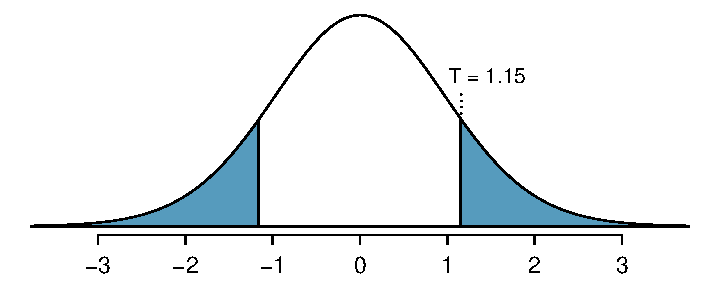
\includegraphics[width=0.7\textwidth]{ch_inference_for_means/figures/pValueOfTwoTailAreaOfExamVersionsWhereDFIs26/pValueOfTwoTailAreaOfExamVersionsWhereDFIs26}
\caption{The $t$ distribution with 26 degrees of freedom. The shaded right tail represents values with $T \geq 1.15$. Because it is a two-sided test, we also shade the corresponding lower tail.}
\label{pValueOfTwoTailAreaOfExamVersionsWhereDFIs26}
\end{figure}

\begin{example}{Identify the p-value using $df = 26$ and provide a conclusion in the context of the case study.}
We examine row $df=26$ in the $t$ table. Because this value is smaller than the value in the left column, the p-value is larger than 0.200 (two tails!). Because the p-value is so large, we do not reject the null hypothesis. That is, the data do not convincingly show that one exam version is more difficult than the other, and the teacher should not be convinced that she should add points to the Version B exam scores.

\index{data!two exam comparison|)}
\end{example}



\subsection{Summary for inference using the $t$ distribution}

%When considering the difference of two means, there are two common cases: the two samples are paired or they are independent. (There are instances where the data are neither paired nor independent, e.g. see blocking in Section~\ref{experimentalDesignPrinciples}.) The paired case was treated in Section~\ref{pairedData}, where the one-sample methods were applied to the differences from the paired observations. We examined the second and more complex scenario in this section.

\textbf{Hypothesis tests.} When applying the $t$ distribution for a hypothesis test, we proceed as follows:
\begin{itemize}
\setlength{\itemsep}{0mm}
\item Write appropriate hypotheses.
\item Verify conditions for using the $t$ distribution.
\begin{itemize}
\item One-sample or differences from paired data: the observations (or differences) must be independent and nearly normal. For larger sample sizes, we can relax the nearly normal requirement, e.g. slight skew is okay for sample sizes of 15, moderate skew for sample sizes of 30, and strong skew for sample sizes of 60.
\item For a difference of means when the data are not paired: each sample mean must separately satisfy the one-sample conditions for the $t$ distribution, and the data in the groups must also be independent.
\end{itemize}
\item Compute the point estimate of interest, the standard error, and the degrees of freedom. For $df$, use $n-1$ for one sample, and for two samples use either statistical software or the smaller of $n_1 - 1$ and $n_2 - 1$.
\item Compute the T score and p-value.
\item Make a conclusion based on the p-value, and write a conclusion in context and in plain language so anyone can understand the result.
\end{itemize}
\noindent\textbf{Confidence intervals.} Similarly, the following is how we generally computed a confidence interval using a $t$ distribution:
\begin{itemize}
\item Verify conditions for using the $t$ distribution. (See above.)
\item Compute the point estimate of interest, the standard error, the degrees of freedom, and $t^{\star}_{df}$.
\item Calculate the confidence interval using the general formula, point estimate $\pm\ t_{df}^{\star} SE$.
\item Put the conclusions in context and in plain language so even non-statisticians can understand the results.
\end{itemize}


\subsection{Examining the standard error formula (special topic)}

\Comment{Made this a special topic section.}

The formula for the standard error of the difference in two means is similar to the formula for other standard errors. Recall that the standard error of a single mean, $\bar{x}_1$, can be approximated by
\begin{eqnarray*}
SE_{\bar{x}_1} = \frac{s_1}{\ \sqrt{n_1}\ }
\end{eqnarray*}
where $s_1$ and $n_1$ represent the sample standard deviation and sample size.

The standard error of the difference of two sample means can be constructed from the standard errors of the separate sample means:
\begin{eqnarray}
SE_{\bar{x}_{1} - \bar{x}_{2}}
	= \sqrt{SE_{\bar{x}_1}^2 + SE_{\bar{x}_2}^2}
	= \sqrt{\frac{s_1^2}{{n_1}} + \frac{s_2^2}{{n_2}}}
\label{seOfDiffOfMeansInTermsOfSEOfIndividualMeans}
\end{eqnarray}
This special relationship follows from probability theory.

\begin{exercise}\label{derivingSEForDiffOfTwoMeansExercise}
Prerequisite: Section~\ref{randomVariablesSection}.
We can rewrite Equation~(\ref{seOfDiffOfMeansInTermsOfSEOfIndividualMeans}) in a different way:
\begin{eqnarray*}
SE_{\bar{x}_{1} - \bar{x}_{2}}^2 = SE_{\bar{x}_1}^2 + SE_{\bar{x}_2}^2
\end{eqnarray*}
Explain where this formula comes from using the ideas of probability theory.\footnote{The standard error squared represents the variance of the estimate. If $X$ and $Y$ are two random variables with variances $\sigma_x^2$ and $\sigma_y^2$, then the variance of $X-Y$ is $\sigma_x^2 + \sigma_y^2$. Likewise, the variance corresponding to $\bar{x}_1 - \bar{x}_2$ is $\sigma_{\bar{x}_1}^2 + \sigma_{\bar{x}_2}^2$. Because $\sigma_{\bar{x}_1}^2$ and $\sigma_{\bar{x}_2}^2$ are just another way of writing $SE_{\bar{x}_1}^2$ and  $SE_{\bar{x}_2}^2$, the variance associated with $\bar{x}_1 - \bar{x}_2$ may be written as $SE_{\bar{x}_1}^2 + SE_{\bar{x}_2}^2$.}
\end{exercise}


\subsection{Pooled standard deviation estimate (special topic)}
\label{pooledStandardDeviations}

Occasionally, two populations will have standard deviations that are so similar that they can be treated as identical. For example, historical data or a well-understood biological mechanism may justify this strong assumption. In such cases, we can make the $t$ distribution approach slightly more precise by using a pooled standard deviation.

The \term{pooled standard deviation} of two groups is a way to use data from both samples to better estimate the standard deviation and standard error. If $s_1^{}$ and $s_2^{}$ are the standard deviations of groups 1 and 2 and there are good reasons to believe that the population standard deviations are equal, then we can obtain an improved estimate of the group variances by pooling their data:
\begin{align*}
s_{pooled}^2 = \frac{s_1^2\times (n_1-1) + s_2^2\times (n_2-1)}{n_1 + n_2 - 2}
\end{align*}
where $n_1$ and $n_2$ are the sample sizes, as before. To use this new statistic, we substitute $s_{pooled}^2$ in place of $s_1^2$ and $s_2^2$ in the standard error formula, and we use an updated formula for the degrees of freedom:
\begin{align*}
df = n_1 + n_2 - 2
\end{align*}

The benefits of pooling the standard deviation are realized through obtaining a better estimate of the standard deviation for each group and using a larger degrees of freedom parameter for the $t$ distribution. Both of these changes may permit a more accurate model of the sampling distribution of $\bar{x}_1 - \bar{x}_2$\Add{, if the standard deviations of the two groups are~equal}.

\Comment{I've updated the title of the caution box below from \emph{Pooling standard deviations should be done only after careful research}.}

\begin{caution}
{Pooling standard deviations only after careful consideration}
{A pooled standard deviation is only appropriate when background research indicates the population standard deviations are nearly equal. When the sample size is large and the condition may be adequately checked with data, the benefits of pooling the standard deviations greatly diminishes.}
\end{caution}
}



%__________________
\section[Comparing many means with ANOVA (special topic)]{Comparing many means with ANOVA\\(special topic)}
\label{anovaAndRegrWithCategoricalVariables}

\index{analysis of variance (ANOVA)|(}

Sometimes we want to compare means across many groups. We might initially think to do pairwise comparisons; for example, if there were three groups, we might be tempted to compare the first mean with the second, then with the third, and then finally compare the second and third means for a total of three comparisons. However, this strategy can be treacherous. If we have many groups and do many comparisons, it is likely that we will eventually find a difference just by chance, even if there is no difference in the populations.

In this section, we will learn a new method called \term{analysis of variance (ANOVA)} and a new test statistic called $F$. ANOVA uses a single hypothesis test to check whether the means across many groups are equal:
\begin{itemize}
\setlength{\itemsep}{0mm}
\item[$H_0$:] The mean outcome is the same across all groups. In statistical notation, $\mu_1 = \mu_2 = \cdots = \mu_k$ where $\mu_i$ represents the mean of the outcome for observations in category $i$.
\item[$H_A$:] At least one mean is different.
\end{itemize}
Generally we must check three conditions on the data before performing ANOVA:
\begin{itemize}
\setlength{\itemsep}{0mm}
\item the observations are independent within and across groups,
\item the data within each group are nearly normal, and
\item the variability across the groups is about equal.
\end{itemize}
When these three conditions are met, we may perform an ANOVA to determine whether the data provide strong evidence against the null hypothesis that all the $\mu_i$ are equal.

\begin{example}{College departments commonly run multiple lectures of the same introductory course each semester because of high demand. Consider a statistics department that runs three lectures of an introductory statistics course. We might like to determine whether there are statistically significant differences in first exam scores in these three classes ($A$, $B$, and $C$). Describe appropriate hypotheses to determine whether there are any differences between the three classes.} \label{firstExampleForThreeStatisticsClassesAndANOVA}
The hypotheses may be written in the following form:
\begin{itemize}
\setlength{\itemsep}{0mm}
\item[$H_0$:] The average score is identical in all lectures. Any observed difference is due to chance. Notationally, we write $\mu_A=\mu_B=\mu_C$.
\item[$H_A$:] The average score varies by class. We would reject the null hypothesis in favor of the alternative hypothesis if there were larger differences among the class averages than what we might expect from chance alone.
\end{itemize}
\end{example}

Strong evidence favoring the alternative hypothesis in ANOVA is described by unusually large differences among the group means. We will soon learn that assessing the variability of the group means relative to the variability among individual observations within each group is key to ANOVA's success.

\begin{example}{Examine Figure~\ref{toyANOVA}. Compare groups I, II, and III. Can you visually determine if the differences in the group centers is due to chance or not? Now compare groups IV, V, and VI. Do these differences appear to be due to chance?}

\begin{figure}[h]
\centering
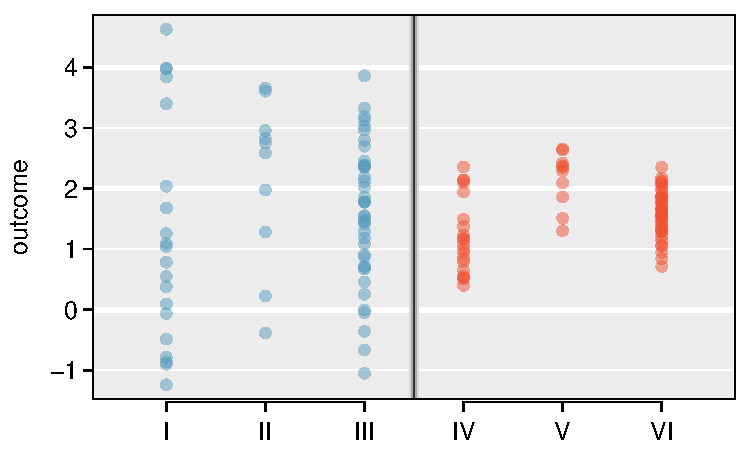
\includegraphics[width=0.65\textwidth]{ch_inference_for_means/figures/toyANOVA/toyANOVA}
\caption{Side-by-side dot plot for the outcomes for six groups.\vspaceB{-3.5mm}}
\label{toyANOVA}
\end{figure}

Any real difference in the means of groups I, II, and III is difficult to discern, because the data within each group are very volatile relative to any differences in the average outcome. On the other hand, it appears there are differences in the centers of groups IV, V, and VI. For instance, group V appears to have a higher mean than that of the other two groups. Investigating groups IV, V, and VI, we see the differences in the groups' centers are noticeable because those differences are large \emph{relative to the variability in the individual observations within each group}.
\end{example}


\subsection{Is batting performance related to player position in MLB?}

\index{data!MLB batting|(}

We would like to discern whether there are real differences between the batting performance of baseball players according to their position: outfielder (\resp{OF}), infielder (\resp{IF}), designated hitter (\resp{DH}), and catcher (\resp{C}). We will use a data set called \data{bat10}, which includes batting records of 327 Major League Baseball (MLB) players from the 2010 season. Six of the 327 cases represented in \data{bat10} are shown in Table~\ref{mlbBat10DataMatrix}, and descriptions for each variable are provided in Table~\ref{mlbBat10Variables}. The measure we will use for the player batting performance (the outcome variable) is on-base percentage (\var{OBP}). The on-base percentage roughly represents the fraction of the time a player successfully gets on base or hits a home run.

\begin{table}[h]
\centering
\begin{tabular}{rlllrrrrrr}
  \hline
 & name & team & position & AB & H & HR &RBI & AVG & OBP \\ 
  \hline
1 & I Suzuki & SEA & OF & 680 & 214 & 6 & 43 & 0.315 & 0.359 \\ 
  2 & D Jeter & NYY & IF & 663 & 179 & 10 & 67 & 0.270 & 0.340 \\ 
  3 & M Young & TEX & IF & 656 & 186 & 21 & 91 & 0.284 & 0.330 \\ 
  $\vdots$ & $\vdots$ & $\vdots$ & $\vdots$ & $\vdots$ & $\vdots$ & $\vdots$ & $\vdots$ \\
  325 & B Molina & SF & C & 202 & 52 & 3 & 17 & 0.257 & 0.312 \\ 
  326 & J Thole & NYM & C & 202 & 56 & 3 & 17 & 0.277 & 0.357 \\ 
  327 & C Heisey & CIN & OF & 201 & 51 & 8 & 21 & 0.254 & 0.324 \\ 
   \hline
\end{tabular}
\caption{Six cases from the \data{bat10} data matrix.\vspaceB{-3mm}}
\label{mlbBat10DataMatrix}
\end{table}

\begin{table}[h]
\centering\small
\begin{tabular}{lp{8.5cm}}
\hline
{\bf variable} & {\bf description} \\
\hline
\var{name} & Player name \\
\var{team} & The abbreviated name of the player's team \\
\var{position} & The player's primary field position (\resp{OF}, \resp{IF}, \resp{DH}, \resp{C}) \\
\var{AB} & Number of opportunities at bat \\
\var{H} & Number of hits \\
\var{HR} & Number of home runs \\
\var{RBI} & Number of runs batted in \\
\var{AVG} & Batting average, which is equal to $\resp{H}/\resp{AB}$ \\
\var{OBP} & On-base percentage, which is roughly equal to the fraction of times a player gets on base or hits a home run \\
\hline
\end{tabular}
\caption{Variables and their descriptions for the \data{bat10} data set.}
\label{mlbBat10Variables}
\end{table}

\begin{exercise} \label{nullHypForOBPAgainstPosition}
The null hypothesis under consideration is the following: $\mu_{\resp{OF}} = \mu_{\resp{IF}} = \mu_{\resp{DH}} = \mu_{\resp{C}}$.
Write the null and corresponding alternative hypotheses in plain language.\footnote{$H_0$: The average on-base percentage is equal across the four positions. $H_A$: The average on-base percentage varies across some (or all) groups.}
\end{exercise}

\begin{example}{The player positions have been divided into four groups: outfield (\resp{OF}), infield (\resp{IF}), designated hitter (\resp{DH}), and catcher (\resp{C}). What would be an appropriate point estimate of the on-base percentage by outfielders, $\mu_{\resp{OF}}$?}
A good estimate of the on-base percentage by outfielders would be the sample average of \var{OBP} for just those players whose position is outfield: $\bar{x}_{OF} = 0.334$.
\end{example}

Table~\ref{mlbHRPerABSummaryTable} provides summary statistics for each group. A side-by-side box plot for the on-base percentage is shown in Figure~\ref{mlbANOVABoxPlot}. Notice that the variability appears to be approximately constant across groups; nearly constant variance across groups is an important assumption that must be satisfied before we consider the ANOVA approach.

\begin{table}[ht]
\centering\small
\begin{tabular}{lrrrr}
\hline
	& \resp{OF} & \resp{IF} & \resp{DH} & \resp{C} \\
\hline
Sample size ($n_i$)	& 120 & 154 & 14 & 39 \\
Sample mean ($\bar{x}_i$)	& 0.334 & 0.332 & 0.348 & 0.323 \\
Sample SD ($s_i$)	& 0.029 & 0.037 & 0.036 & 0.045 \\
\hline
\end{tabular}
\caption{Summary statistics of on-base percentage, split by player position.}
\label{mlbHRPerABSummaryTable}
\end{table}

\begin{figure}
\centering
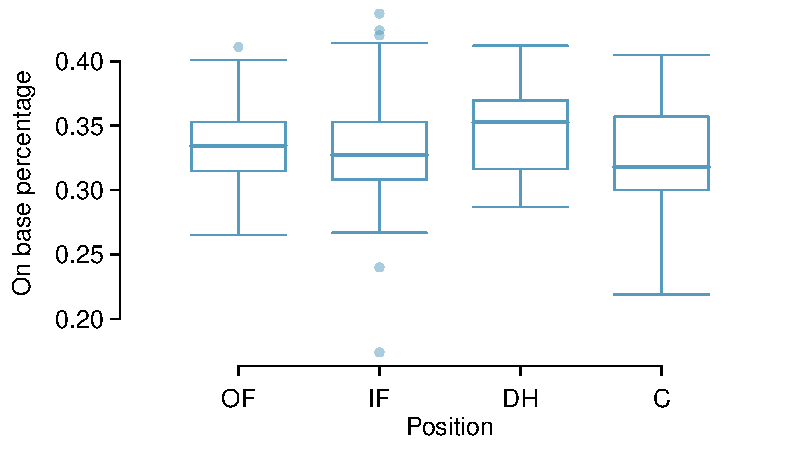
\includegraphics[width=0.85\textwidth]{ch_inference_for_means/figures/mlbANOVA/mlbANOVABoxPlot}
\caption{Side-by-side box plot of the on-base percentage for 327 players across four groups. There is one prominent outlier visible in the infield group, but with 154 observations in the infield group, this outlier is not a concern.}
\label{mlbANOVABoxPlot}
\end{figure}

\begin{example}{The largest difference between the sample means is between the designated hitter and the catcher positions. Consider again the original hypotheses:
\begin{itemize}
\setlength{\itemsep}{0mm}
\item[$H_0$:] $\mu_{\resp{OF}} = \mu_{\resp{IF}} = \mu_{\resp{DH}} = \mu_{\resp{C}}$
\item[$H_A$:] The average on-base percentage ($\mu_i$) varies across some (or all) groups.
\end{itemize}
Why might it be inappropriate to run the test by simply estimating whether the difference of $\mu_{\var{DH}}$ and $\mu_{\resp{C}}$ is statistically significant at a 0.05 significance level?}
\label{multipleComparisonExampleThatIncludesDiscussionOfClassrooms}
The primary issue here is that we are inspecting the data before picking the groups that will be compared. It is inappropriate to examine all data by eye (informal testing) and only afterwards decide which parts to formally test. This is called \term{data snooping} or \term{data fishing}. Naturally we would pick the groups with the large differences for the formal test, leading to an inflation in the Type 1 Error rate. To understand this better, let's consider a slightly different problem.

Suppose we are to measure the aptitude for students in 20 classes in a large elementary school at the beginning of the year. In this school, all students are randomly assigned to classrooms, so any differences we observe between the classes at the start of the year are completely due to chance. However, with so many groups, we will probably observe a few groups that look rather different from each other. If we select only these classes that look so different, we will probably make the wrong conclusion that the assignment wasn't random. While we might only formally test differences for a few pairs of classes, we informally evaluated the other classes by eye before choosing the most extreme cases for a comparison.
\end{example}

For additional information on the ideas expressed in Example~\ref{multipleComparisonExampleThatIncludesDiscussionOfClassrooms}, we recommend reading about the \term{prosecutor's fallacy}.\footnote{See, for example, \href{http://www.stat.columbia.edu/~cook/movabletype/archives/2007/05/the_prosecutors.html}{www.stat.columbia.edu/$\sim$cook/movabletype/archives/2007/05/the\_prosecutors.html}.}

In the next section we will learn how to use the $F$ statistic and ANOVA to test whether observed differences in sample means could have happened just by chance even if there was no difference in the respective population means.


\subsection{Analysis of variance (ANOVA) and the F test}

The method of analysis of variance in this context focuses on answering one question: is the variability in the sample means so large that it seems unlikely to be from chance alone? This question is different from earlier testing procedures since we will \emph{simultaneously} consider many groups, and evaluate whether their sample means differ more than we would expect from natural variation. We call this variability the \term{mean square between groups ($MSG$)}, and it has an associated degrees of freedom, $df_{G}=k-1$ when there are $k$ groups. The $MSG$ can be thought of as a scaled variance formula for means. If the null hypothesis is true, any variation in the sample means is due to chance and shouldn't be too large. Details of $MSG$ calculations are provided in the footnote,\footnote{Let $\bar{x}$ represent the mean of outcomes across all groups. Then the mean square between groups is computed as
\begin{align*}
MSG = \frac{1}{df_{G}}SSG = \frac{1}{k-1}\sum_{i=1}^{k} n_{i}\left(\bar{x}_{i} - \bar{x}\right)^2
\end{align*}
where $SSG$ is called the \term{sum of squares between groups} and $n_{i}$ is the sample size of group $i$.} however, we typically use software for these computations.

The mean square between the groups is, on its own, quite useless in a hypothesis test. We need a benchmark value for how much variability should be expected among the sample means if the null hypothesis is true. To this end, we compute a pooled variance estimate, often abbreviated as the \term{mean square error ($MSE$)}, which has an associated degrees of freedom value $df_E=n-k$. It is helpful to think of $MSE$ as a measure of the variability within the groups. Details of the computations of the $MSE$ are provided in the footnote\footnote{Let $\bar{x}$ represent the mean of outcomes across all groups. Then the \term{sum of squares total ($SST$)} is computed as
\begin{align*}
SST = \sum_{i=1}^{n} \left(x_{i} - \bar{x}\right)^2
\end{align*}
where the sum is over all observations in the data set. Then we compute the \term{sum of squared errors ($SSE$)} in one of two equivalent ways:
\begin{align*}
SSE &= SST - SSG \\
	&= (n_1-1)s_1^2 + (n_2-1)s_2^2 + \cdots + (n_k-1)s_k^2
\end{align*}
where $s_i^2$ is the sample variance (square of the standard deviation) of the residuals in group $i$. Then the $MSE$ is the standardized form of $SSE$: $MSE = \frac{1}{df_{E}}SSE$.} for interested readers.

When the null hypothesis is true, any differences among the sample means are only due to chance, and the $MSG$ and $MSE$ should be about equal. As a test statistic for ANOVA, we examine the fraction of $MSG$ and $MSE$:
\begin{align} \label{formulaForTheFStatistic}
F = \frac{MSG}{MSE}
\end{align}
The $MSG$ represents a measure of the between-group variability, and $MSE$ measures the variability within each of the groups.

\begin{exercise}
For the baseball data, $MSG = 0.00252$ and $MSE=0.00127$. Identify the degrees of freedom associated with MSG and MSE and verify the $F$ statistic is approximately 1.994.\footnote{There are $k=4$ groups, so $df_{G} = k-1 = 3$. There are $n = n_1 + n_2 + n_3 + n_4 = 327$ total observations, so $df_{E} = n - k = 323$. Then the $F$ statistic is computed as the ratio of $MSG$ and $MSE$: $F = \frac{MSG}{MSE} = \frac{0.00252}{0.00127} = 1.984 \approx 1.994$. ($F=1.994$ was computed by using values for $MSG$ and $MSE$ that were not rounded.)}
\end{exercise}

We can use the $F$ statistic to evaluate the hypotheses in what is called an \term{F test}. A p-value can be computed from the $F$ statistic using an $F$ distribution, which has two associated parameters: $df_{1}$ and $df_{2}$. For the $F$ statistic in ANOVA, $df_{1} = df_{G}$ and $df_{2}= df_{E}$. An $F$ distribution with 3 and 323 degrees of freedom, corresponding to the $F$ statistic for the baseball hypothesis test, is shown in Figure~\ref{fDist3And323}.

\begin{figure}[ht]
\centering
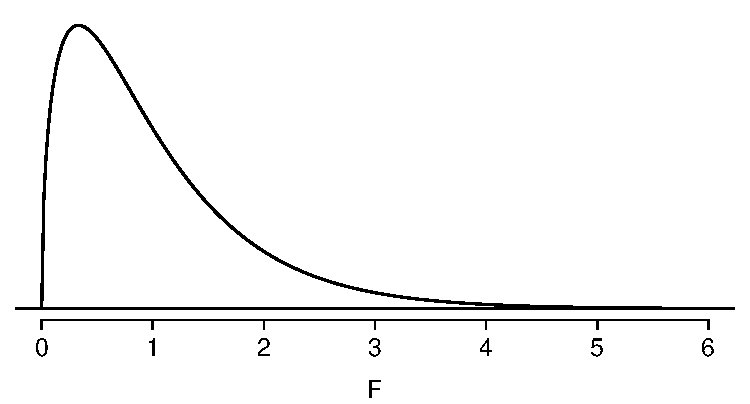
\includegraphics[width=0.7\textwidth]{ch_inference_for_means/figures/fDist3And323/fDist3And323}
\caption{An $F$ distribution with $df_1=3$ and $df_2=323$.}
\label{fDist3And323}
\end{figure}

The larger the observed variability in the sample means ($MSG$) relative to the within-group observations ($MSE$), the larger $F$ will be and the stronger the evidence against the null hypothesis. Because larger values of $F$ represent stronger evidence against the null hypothesis, we use the upper tail of the distribution to compute a p-value.

\begin{termBox}{\tBoxTitle{The $F$ statistic and the $F$ test}
Analysis of variance (ANOVA) is used to test whether the mean outcome differs across 2 or more groups. ANOVA uses a test statistic $F$, which represents a standardized ratio of variability in the sample means relative to the variability within the groups. If $H_0$ is true and the model assumptions are satisfied, the statistic $F$ follows an $F$ distribution with parameters $df_{1}=k-1$ and $df_{2}=n-k$. The upper tail of the $F$ distribution is used to represent the p-value.}
\end{termBox}

\begin{exercise}\label{describePValueAreaForFDistributionInMLBOBPExample}
The test statistic for the baseball example is $F=1.994$. Shade the area corresponding to the p-value in Figure~\ref{fDist3And323}. \footnote{\ \vspace{-4mm}\\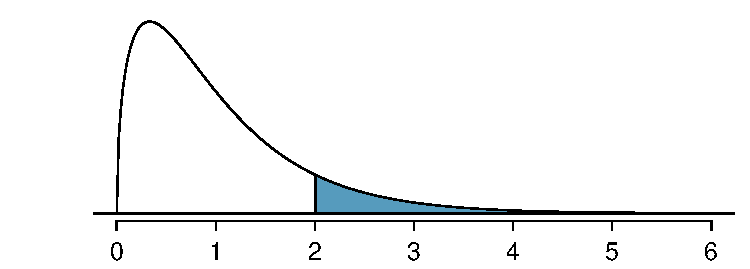
\includegraphics[height=20mm]{ch_inference_for_means/figures/fDist3And323/fDist3And323Shaded}}
\end{exercise}

\begin{example}{The p-value corresponding to the shaded area in the solution of Exercise~\ref{describePValueAreaForFDistributionInMLBOBPExample} is equal to about 0.115. Does this provide strong evidence against the null hypothesis?}
The p-value is larger than 0.05, indicating the evidence is not strong enough to reject the null hypothesis at a significance level of 0.05. That is, the data do not provide strong evidence that the average on-base percentage varies by player's primary field position.
\end{example}


\subsection{Reading an ANOVA table from software}

The calculations required to perform an ANOVA by hand are tedious and prone to human error. For these reasons, it is common to use statistical software to calculate the $F$ statistic and p-value.

An ANOVA can be summarized in a table very similar to that of a regression summary, which we will see in \MultipleRegressionChapter{Chapters~\ref{linRegrForTwoVar} and~\ref{multipleAndLogisticRegression}}{Chapter~\ref{linRegrForTwoVar}}. Table~\ref{anovaSummaryTableForOBPAgainstPosition} shows an ANOVA summary to test whether the mean of on-base percentage varies by player positions in the MLB. Many of these values should look familiar; in particular, the $F$ test statistic and p-value can be retrieved from the last columns.

\begin{table}[ht]
\centering
\begin{tabular}{lrrrrr}
  \hline
 & Df & Sum Sq & Mean Sq & F value & Pr($>$F) \\ 
  \hline
position & 3 & 0.0076 & 0.0025 & 1.9943 & 0.1147 \\ 
  Residuals & 323 & 0.4080 & 0.0013 &  &  \\    \hline
\multicolumn{6}{r}{$s_{pooled} = 0.036$ on $df=323$}
\end{tabular}
\caption{ANOVA summary for testing whether the average on-base percentage differs across player positions.}
\label{anovaSummaryTableForOBPAgainstPosition}
\end{table}


\subsection{Graphical diagnostics for an ANOVA analysis}

There are three conditions we must check for an ANOVA analysis: all observations must be independent, the data in each group must be nearly normal, and the variance within each group must be approximately equal.

\begin{description}
\item[Independence.] If the data are a simple random sample from less than 10\% of the population, this condition is satisfied. For processes and experiments, carefully consider whether the data may be independent (e.g. no pairing). For example, in the MLB data, the data were not sampled. However, there are not obvious reasons why independence would not hold for most or all observations.
\item[Approximately normal.] As with one- and two-sample testing for means, the normality assumption is especially important when the sample size is quite small. The normal probability plots for each group of the MLB data are shown in Figure~\ref{mlbANOVADiagNormalityGroups}; there is some deviation from normality for infielders, but this isn't a substantial concern since there are about 150 observations in that group and the outliers are not extreme. Sometimes in ANOVA there are so many groups or so few observations per group that checking normality for each group isn't reasonable. See the footnote\footnote{First calculate the \termsub{residuals}{residual} of the baseball data, which are calculated by taking the observed values and subtracting the corresponding group means. For example, an outfielder with OBP of 0.405 would have a residual of $0.405 - \bar{x}_{OF} = 0.071$. Then to check the normality condition, create a normal probability plot using all the residuals simultaneously.} for guidance on how to handle such instances.

\begin{figure}[hhh]
\centering
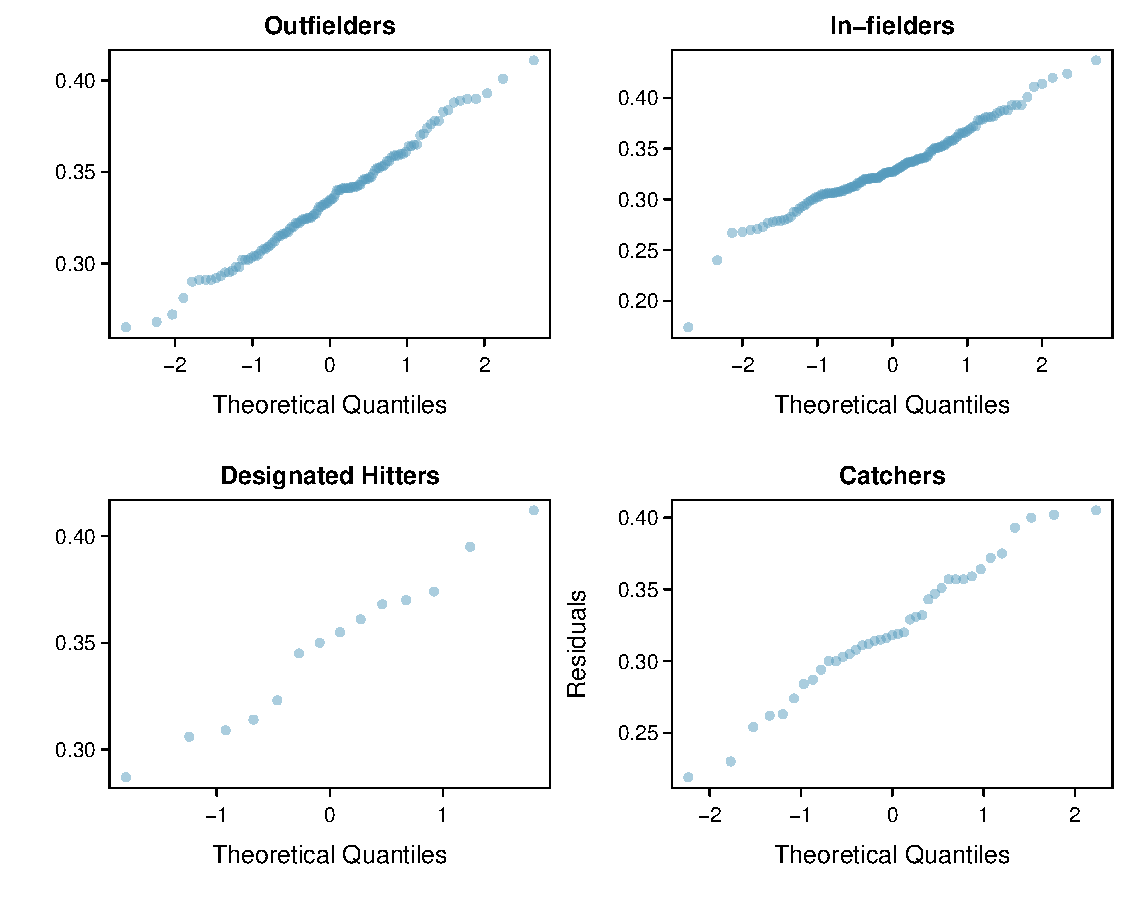
\includegraphics[width=\textwidth]{ch_inference_for_means/figures/mlbANOVA/mlbANOVADiagNormalityGroups}
\caption{Normal probability plot of OBP for each field position.}
\label{mlbANOVADiagNormalityGroups}
\end{figure}

\item[Constant variance.] The last assumption is that the variance in the groups is about equal from one group to the next. This assumption can be checked by examining a side-by-side box plot of the outcomes across the groups, as in Figure~\vref{mlbANOVABoxPlot}. In this case, the variability is similar in the four groups but not identical. We see in Table~\vref{mlbHRPerABSummaryTable} that the standard deviation varies a bit from one group to the next. Whether these differences are from natural variation is unclear, so we should report this uncertainty with the final results.

\index{data!MLB batting|)}

\end{description}

\begin{caution}
{Diagnostics for an ANOVA analysis}
{Independence is always important to an ANOVA analysis. The normality condition is very important when the sample sizes for each group are relatively small. The constant variance condition is especially important when the sample sizes differ between groups.}
\end{caution}


\subsection{Multiple comparisons and controlling Type 1 Error rate}
\label{multipleComparisonsAndControllingTheType1ErrorRate}

\index{significance level!multiple comparisons|(}

When we reject the null hypothesis in an ANOVA analysis, we might wonder, which of these groups have different means? To answer this question, we compare the means of each possible pair of groups. For instance, if there are three groups and there is strong evidence that there are some differences in the group means, there are three comparisons to make: group 1 to group 2, group 1 to group 3, and group 2 to group 3. These comparisons can be accomplished using a two-sample $t$ test, but we use a modified significance level and a pooled estimate of the standard deviation across groups. Usually this pooled standard deviation can be found in the ANOVA table, e.g. along the bottom of Table~\ref{anovaSummaryTableForOBPAgainstPosition}.

\begin{example}{Example~\vref{firstExampleForThreeStatisticsClassesAndANOVA} discussed three statistics lectures, all taught during the same semester. Table~\ref{summaryStatisticsForClassTestData} shows summary statistics for these three courses, and a side-by-side box plot of the data is shown in Figure~\ref{classDataSBSBoxPlot}. We would like to conduct an ANOVA for these data. Do you see any deviations from the three conditions for ANOVA?}
In this case (like many others) it is difficult to check independence in a rigorous way. Instead, the best we can do is use common sense to consider reasons the assumption of independence may not hold. For instance, the independence assumption may not be reasonable if there is a star teaching assistant that only half of the students may access; such a scenario would divide a class into two subgroups. No such situations were evident for these particular data, and we believe that independence is acceptable.

The distributions in the side-by-side box plot appear to be roughly symmetric and show no noticeable outliers.

The box plots show approximately equal variability, which can be verified in Table~\ref{summaryStatisticsForClassTestData}, supporting the constant variance assumption.
\end{example}

\begin{table}
\centering
\begin{tabular}{lrrr}
  \hline
Class $i$	& A	& B	& C \\ 
  \hline
$n_i$		& 58	& 55	& 51 \\ 
$\bar{x}_i$	& 75.1	& 72.0	& 78.9 \\ 
$s_i$		& 13.9	& 13.8	& 13.1 \\ 
\hline
\end{tabular}
\caption{Summary statistics for the first midterm scores in three different lectures of the same course.}
\label{summaryStatisticsForClassTestData}
\end{table}

\begin{figure}
\centering
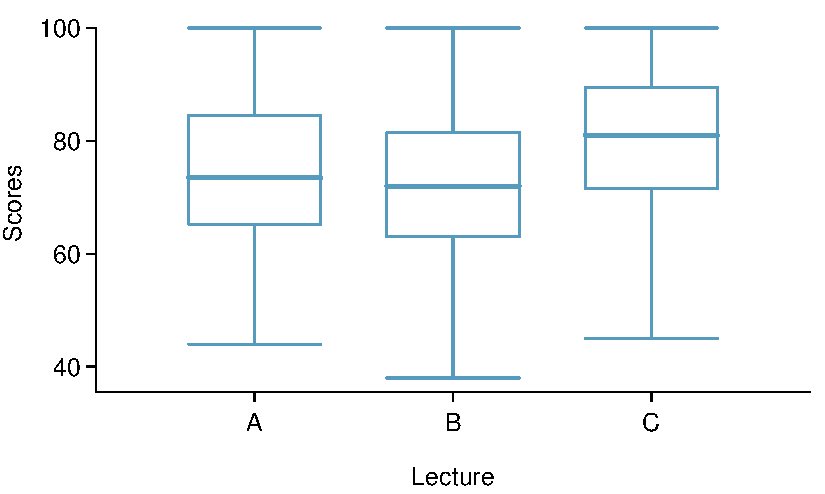
\includegraphics[width=0.8\textwidth]{ch_inference_for_means/figures/classData/classDataSBSBoxPlot}
\caption{Side-by-side box plot for the first midterm scores in three different  lectures of the same course.}
\label{classDataSBSBoxPlot}
\end{figure}

\begin{exercise} \label{exerExaminingAnovaSummaryTableForMidtermData}
An ANOVA was conducted for the midterm data, and summary results are shown in Table~\ref{anovaSummaryTableForMidtermData}. What should we conclude?\footnote{The p-value of the test is 0.0330, less than the default significance level of 0.05. Therefore, we reject the null hypothesis and conclude that the difference in the average midterm scores are not due to chance.}
\end{exercise}

\begin{table}
\centering
\begin{tabular}{lrrrrr}
  \hline
 & Df & Sum Sq & Mean Sq & F value & Pr($>$F) \\ 
  \hline
lecture & 2 & 1290.11 & 645.06 & 3.48 & 0.0330 \\ 
  Residuals & 161 & 29810.13 & 185.16 &  &  \\ 
   \hline
\multicolumn{6}{r}{$s_{pooled}=13.61$ on $df=161$}
\end{tabular}
\caption{ANOVA summary table for the midterm data.\vspaceB{-5mm}}
\label{anovaSummaryTableForMidtermData}
\end{table}

There is strong evidence that the different means in each of the three classes is not simply due to chance. We might wonder, which of the classes are actually different? As discussed in earlier chapters, a two-sample $t$ test could be used to test for differences in each possible pair of groups. However, one pitfall was discussed in Example~\vref{multipleComparisonExampleThatIncludesDiscussionOfClassrooms}: when we run so many tests, the Type~1 Error rate increases. This issue is resolved by using a modified significance level. \vspaceB{-1mm}

\begin{termBox}{\tBoxTitle{Multiple comparisons and the Bonferroni correction for $\alpha$}
The scenario of testing many pairs of groups is called \term{multiple comparisons}. The \term{Bonferroni correction} suggests that a more stringent significance level is more appropriate for these tests:
\begin{align*}
\alpha^* = \alpha / K
\end{align*}
where $K$ is the number of comparisons being considered (formally or informally). If there are $k$ groups, then usually all possible pairs are compared and $K=\frac{k(k-1)}{2}$.}
\end{termBox}

\begin{example}{In Exercise~\ref{exerExaminingAnovaSummaryTableForMidtermData}, you found strong evidence of differences in the average midterm grades between the three lectures. Complete the three possible pairwise comparisons using the Bonferroni correction and report any differences.} \label{multipleComparisonsOfThreeStatClasses}
We use a modified significance level of $\alpha^* = 0.05/3 = 0.0167$. Additionally, we use the pooled estimate of the standard deviation: $s_{pooled}=13.61$ on $df=161$, which is provided in the ANOVA summary table.

Lecture A versus Lecture B: The estimated difference and standard error are, respectively,
\begin{align*}
\bar{x}_A - \bar{x}_{B} &= 75.1 - 72 = 3.1
	&SE = \sqrt{\frac{13.61^2}{58} + \frac{13.61^2}{55}} &= 2.56
\end{align*}
(See Section~\vref{pooledStandardDeviations} for additional details.) This results in a $T$ score of 1.21 on $df = 161$ (we use the $df$ associated with $s_{pooled}$). Statistical software was used to precisely identify the two-tailed p-value since the modified significance of 0.0167 is not found in the $t$ table. The p-value (0.228) is larger than $\alpha^*=0.0167$, so there is not strong evidence of a difference in the means of lectures A and B.

Lecture A versus Lecture C: The estimated difference and standard error are 3.8 and 2.61, respectively. This results in a $T$ score of 1.46 on $df = 161$ and a two-tailed p-value of 0.1462. This p-value is larger than $\alpha^*$, so there is not strong evidence of a difference in the means of lectures A and C.

Lecture B versus Lecture C: The estimated difference and standard error are 6.9 and 2.65, respectively. This results in a $T$ score of 2.60 on $df = 161$ and a two-tailed p-value of 0.0102. This p-value is smaller than $\alpha^*$. Here we find strong evidence of a difference in the means of lectures B and C.
\end{example}

We might summarize the findings of the analysis from Example~\ref{multipleComparisonsOfThreeStatClasses} using the following notation:
\begin{align*}
\mu_A &\stackrel{?}{=} \mu_B
	&\mu_A &\stackrel{?}{=} \mu_C
	&\mu_B &\neq \mu_C
\end{align*}
The midterm mean in lecture A is not statistically distinguishable from those of lectures B or C. However, there is strong evidence that lectures B and C are different. In the first two pairwise comparisons, we did not have sufficient evidence to reject the null hypothesis. Recall that failing to reject $H_0$ does not imply $H_0$ is true.

\begin{caution}
{Sometimes an ANOVA will reject the null but no groups will have statistically significant differences}
{It is possible to reject the null hypothesis using ANOVA and then to not subsequently identify differences in the pairwise comparisons. However, \emph{this does not invalidate the ANOVA conclusion}. It only means we have not been able to successfully identify which groups differ in their means.}
\end{caution}

The ANOVA procedure examines the big picture: it considers all groups simultaneously to decipher whether there is evidence that some difference exists. Even if the test indicates that there is strong evidence of differences in group means, identifying with high confidence a specific difference as statistically significant is more difficult.

Consider the following analogy: we observe a Wall Street firm that makes large quantities of money based on predicting mergers. Mergers are generally difficult to predict, and if the prediction success rate is extremely high, that may be considered sufficiently strong evidence to warrant investigation by the Securities and Exchange Commission (SEC). While the SEC may be quite certain that there is insider trading taking place at the firm, the evidence against any single trader may not be very strong. It is only when the SEC considers all the data that they identify the pattern. This is effectively the strategy of ANOVA: stand back and consider all the groups simultaneously.

\index{significance level!multiple comparisons|)}
\index{analysis of variance (ANOVA)|)}

